% Options for packages loaded elsewhere
% Options for packages loaded elsewhere
\PassOptionsToPackage{unicode}{hyperref}
\PassOptionsToPackage{hyphens}{url}
%
\documentclass[
  ignorenonframetext,
]{beamer}
\newif\ifbibliography
\usepackage{pgfpages}
\setbeamertemplate{caption}[numbered]
\setbeamertemplate{caption label separator}{: }
\setbeamercolor{caption name}{fg=normal text.fg}
\beamertemplatenavigationsymbolsempty
% remove section numbering
\setbeamertemplate{part page}{
  \centering
  \begin{beamercolorbox}[sep=16pt,center]{part title}
    \usebeamerfont{part title}\insertpart\par
  \end{beamercolorbox}
}
\setbeamertemplate{section page}{
  \centering
  \begin{beamercolorbox}[sep=12pt,center]{section title}
    \usebeamerfont{section title}\insertsection\par
  \end{beamercolorbox}
}
\setbeamertemplate{subsection page}{
  \centering
  \begin{beamercolorbox}[sep=8pt,center]{subsection title}
    \usebeamerfont{subsection title}\insertsubsection\par
  \end{beamercolorbox}
}
% Prevent slide breaks in the middle of a paragraph
\widowpenalties 1 10000
\raggedbottom
\AtBeginPart{
  \frame{\partpage}
}
\AtBeginSection{
  \ifbibliography
  \else
    \frame{\sectionpage}
  \fi
}
\AtBeginSubsection{
  \frame{\subsectionpage}
}
\usepackage{iftex}
\ifPDFTeX
  \usepackage[T1]{fontenc}
  \usepackage[utf8]{inputenc}
  \usepackage{textcomp} % provide euro and other symbols
\else % if luatex or xetex
  \usepackage{unicode-math} % this also loads fontspec
  \defaultfontfeatures{Scale=MatchLowercase}
  \defaultfontfeatures[\rmfamily]{Ligatures=TeX,Scale=1}
\fi
\usepackage{lmodern}

\usetheme[]{Madrid}
\ifPDFTeX\else
  % xetex/luatex font selection
\fi
% Use upquote if available, for straight quotes in verbatim environments
\IfFileExists{upquote.sty}{\usepackage{upquote}}{}
\IfFileExists{microtype.sty}{% use microtype if available
  \usepackage[]{microtype}
  \UseMicrotypeSet[protrusion]{basicmath} % disable protrusion for tt fonts
}{}
\makeatletter
\@ifundefined{KOMAClassName}{% if non-KOMA class
  \IfFileExists{parskip.sty}{%
    \usepackage{parskip}
  }{% else
    \setlength{\parindent}{0pt}
    \setlength{\parskip}{6pt plus 2pt minus 1pt}}
}{% if KOMA class
  \KOMAoptions{parskip=half}}
\makeatother


\usepackage{longtable,booktabs,array}
\newcounter{none} % for unnumbered tables
\usepackage{calc} % for calculating minipage widths
\usepackage{caption}
% Make caption package work with longtable
\makeatletter
\def\fnum@table{\tablename~\thetable}
\makeatother
\usepackage{graphicx}
\makeatletter
\newsavebox\pandoc@box
\newcommand*\pandocbounded[1]{% scales image to fit in text height/width
  \sbox\pandoc@box{#1}%
  \Gscale@div\@tempa{\textheight}{\dimexpr\ht\pandoc@box+\dp\pandoc@box\relax}%
  \Gscale@div\@tempb{\linewidth}{\wd\pandoc@box}%
  \ifdim\@tempb\p@<\@tempa\p@\let\@tempa\@tempb\fi% select the smaller of both
  \ifdim\@tempa\p@<\p@\scalebox{\@tempa}{\usebox\pandoc@box}%
  \else\usebox{\pandoc@box}%
  \fi%
}
% Set default figure placement to htbp
\def\fps@figure{htbp}
\makeatother





\setlength{\emergencystretch}{3em} % prevent overfull lines

\providecommand{\tightlist}{%
  \setlength{\itemsep}{0pt}\setlength{\parskip}{0pt}}



 


\makeatletter
\@ifpackageloaded{caption}{}{\usepackage{caption}}
\AtBeginDocument{%
\ifdefined\contentsname
  \renewcommand*\contentsname{Table of contents}
\else
  \newcommand\contentsname{Table of contents}
\fi
\ifdefined\listfigurename
  \renewcommand*\listfigurename{List of Figures}
\else
  \newcommand\listfigurename{List of Figures}
\fi
\ifdefined\listtablename
  \renewcommand*\listtablename{List of Tables}
\else
  \newcommand\listtablename{List of Tables}
\fi
\ifdefined\figurename
  \renewcommand*\figurename{Figure}
\else
  \newcommand\figurename{Figure}
\fi
\ifdefined\tablename
  \renewcommand*\tablename{Table}
\else
  \newcommand\tablename{Table}
\fi
}
\@ifpackageloaded{float}{}{\usepackage{float}}
\floatstyle{ruled}
\@ifundefined{c@chapter}{\newfloat{codelisting}{h}{lop}}{\newfloat{codelisting}{h}{lop}[chapter]}
\floatname{codelisting}{Listing}
\newcommand*\listoflistings{\listof{codelisting}{List of Listings}}
\makeatother
\makeatletter
\makeatother
\makeatletter
\@ifpackageloaded{caption}{}{\usepackage{caption}}
\@ifpackageloaded{subcaption}{}{\usepackage{subcaption}}
\makeatother

\usepackage{bookmark}
\IfFileExists{xurl.sty}{\usepackage{xurl}}{} % add URL line breaks if available
\urlstyle{same}
\hypersetup{
  pdftitle={Z-residuals: A Versatile Diagnostic Framework for Bayesian Models},
  hidelinks,
  pdfcreator={LaTeX via pandoc}}


\title{\texorpdfstring{Z-residuals: A Versatile Diagnostic Framework for
Bayesian
Models}{Z-residuals: A Versatile Diagnostic Framework for Bayesian Models}}
\author{}
\date{}

\begin{document}
\frame{\titlepage}


\begin{frame}{Outline}
\protect\phantomsection\label{outline}
\$\$ \% --- LaTeX Packages --- \% --- LaTeX Packages ---

\usepackage{amsmath}
\usepackage{amsthm}

\% For bold math symbols

\usepackage{graphicx}

\% For including images

\usepackage{xcolor}

\% Required for \highlight

\usepackage{xspace}

\% Required for commands like \nref

\usepackage{tikz}

\%\usetikzlibrary{arrows.meta} \%

\usepackage{mathtools}

\%

\usepackage{filecontents}
\usepackage{booktabs}

\%

\usepackage{placeins}
\usepackage{hyperref}
        \hypersetup{
          colorlinks=true,
          linkcolor=blue,
          urlcolor=blue,
          citecolor=blue
        }
\usepackage{etoolbox}

\setlength{\bibsep}{5pt plus 5pt} \% space BETWEEN items \% For tighter
lines WITHIN each item:

\usepackage{setspace}
\AtBeginEnvironment{thebibliography}{\setstretch{1.05}}

\newcommand{\bm}[1]{\boldsymbol{#1}}

\% Maps \bm to \boldsymbol

\% --- Custom Commands ---

\% Acronyms and Custom Text \newcommand{\CVIC}{\text{CVIC}}
\newcommand{\deviance}{\text{dev}} \newcommand{\dpois}{\text{dpois}}
\newcommand{\ic}{\text{ic}} \newcommand{\nmsp}{\text{\scriptsize NMSP}}
\newcommand{\nrsp}{\text{\scriptsize NRSP}}
\newcommand{\pmin}{p_{\text{\scriptsize min}}}
\newcommand{\pp}{\text{pp}} \newcommand{\nref}{[\textbf{references}]}
\newcommand{\SP}{survival probability\xspace}
\newcommand{\SPs}{survival probabilities\xspace}
\newcommand{\svf}{S_{i}(\cdot)} \newcommand{\unif}[0]{\text{Unif}}
\newcommand{\rsp}[0]{\text{RSP}} \newcommand{\msp}[0]{\text{MSP}}
\newcommand{\PPP}[0]{\text{PPP}} \newcommand{\PPPs}[0]{\text{PPPs}}
\newcommand{\PPC}[0]{\text{PPC}} \newcommand{\bU}[0]{\bm{U}}
\newcommand{\pv}[0]{\mathcal{P}}

\% Math Symbols (Bold) \newcommand{\btheta}[0]{\bm{\theta}}
\newcommand{\bTheta}[0]{\bm{\Theta}} \newcommand{\bx}[0]{\bm{x}}
\newcommand{\by}[0]{\bm{y}} \newcommand{\bY}[0]{\bm{Y}}
\newcommand{\bbeta}{\bm{\beta}} \newcommand{\bBeta}{\bm{\Beta}}
\newcommand{\blambda}{\bm{\lambda}} \newcommand{\bmu}{\bm{\mu}}
\newcommand{\bphi}{\bm{\phi}} \newcommand{\bp}{\bm{p}}
\newcommand{\bsgm}{\bm{\sigma}} \newcommand{\hu}[0]{\pi^o_{i}}
\newcommand{\mhu}[0]{\pi^o} \% General Superscripts and Subscripts
\newcommand{\obs}[0]{^{\text{obs}}} \newcommand{\sobs}[0]{^{\text{obs}}}
\newcommand{\post}[0]{^{\text{Post}}} \newcommand{\cv}[0]{^{\text{CV}}}
\newcommand{\iscv}[0]{^{\text{ISCV}}} \newcommand{\supt}[0]{^{(t)}}
\newcommand{\mci}{^{(t)}} \% Kept as it has a different name from ^{(t)}
\newcommand{\mcs}{^{(s)}} \newcommand{\rep}{^{\text{rep}}}
\newcommand{\ppc}{_{\text{ppc}}} \newcommand{\noi}{_{-i}}
\newcommand{\wi}{_{1:n}} \newcommand{\IS}{^{\text{\scriptsize IS}}}

\% Compound Superscripts for Z-residuals
\newcommand{\rspp}[0]{^{\text{Post-RSP}}}
\newcommand{\mspp}[0]{^{\text{Post-MSP}}}
\newcommand{\rspis}[0]{^{\text{ISCV-RSP}}}
\newcommand{\mspis}[0]{^{\text{ISCV-MSP}}}
\newcommand{\rsppost}{^{\text{Post-RSP }}} \% From first block
\newcommand{\rspiscv}{^{\text{ISCV-RSP}}} \% From first block
\newcommand{\E}{\mathbb{E}}
\newcommand{\Epost}{\mathbb{E}_{\btheta\,|\,\by}}
\newcommand{\Ecv}{\mathbb{E}_{\btheta\,|\,\by_{-i}}}
\newcommand{\highlight}[1]{\textcolor{blue}{#1}}
\newcommand{\pvalue}[0]{$p$-value\xspace}
\newcommand{\pvalues}[0]{$p$-values\xspace}
\newcommand{\norm}[1]{\left\lVert#1\right\rVert}

\newcommand{\textred}[1]{\textcolor{orange}{#1}}

\$\$

\begin{enumerate}
\item
  \textbf{Introduction \& Motivation}

  \begin{itemize}
  \tightlist
  \item
    The Diagnostic Gap in Bayesian Modeling
  \item
    Limitations of Posterior Predictive Checks (PPC)
  \end{itemize}
\item
  \textbf{Methodology: The Z-residual Framework}

  \begin{itemize}
  \tightlist
  \item
    Randomized Survival Probability (RSP)
  \item
    Posterior and ISCV Z-residuals
  \item
    Asymptotic Guarantees
  \end{itemize}
\item
  \textbf{Simulation Studies}

  \begin{itemize}
  \tightlist
  \item
    Continuous Inverse Gaussian Regression
  \item
    Discrete Hurdle Negative Binomial Regression
  \end{itemize}
\item
  \textbf{Application to a Zero-inflated Dolphin-Sighting Dataset}
\item
  \textbf{Conclusion \& Future Directions}
\end{enumerate}
\end{frame}

\section{1. Introduction \& Motivation}\label{introduction-motivation}

\begin{frame}{The Central Challenge}
\protect\phantomsection\label{the-central-challenge}
\begin{itemize}
\tightlist
\item
  \textbf{Model Correctness:} Verifying model correctness is a central
  challenge in modern statistics.
\item
  \textbf{Frequentist Diagnostics:}

  \begin{itemize}
  \tightlist
  \item
    Rely heavily on observation-level residual diagnostics.
  \item
    Enable visual checks (QQ plots, scatterplots).
  \item
    Facilitate formal structural tests (Ramsey's RESET, Box-Ljung,
    Breusch-Pagan).
  \end{itemize}
\item
  \textbf{The Gap in Bayesian Modeling:}

  \begin{itemize}
  \tightlist
  \item
    This comprehensive suite of observation-level residual diagnostics
    is largely unavailable for general Bayesian models.
  \item
    We need tools for granular residual \emph{diagnostics}, not just
    overall model \emph{checking}.
  \end{itemize}
\end{itemize}
\end{frame}

\begin{frame}{Posterior Predictive Checks (PPC)}
\protect\phantomsection\label{posterior-predictive-checks-ppc}
\begin{itemize}
\tightlist
\item
  Currently the most widely used tool for Bayesian model assessment.
\item
  \textbf{Goal:} Evaluate consistency between observed data
  \(\mathbf{y}\) and replicated data \(\mathbf{y}^{\text{rep}}\) drawn
  from the posterior predictive distribution.
\item
  \textbf{Mechanism:} Summarized by a PPC \(p\)-value:
  \[ P_B = P(T(\mathbf{y}^{\text{rep}}, \boldsymbol{\theta}) > T(\mathbf{y}, \boldsymbol{\theta}) \mid \mathbf{y}) \]
  where \(T\) is a user-specified discrepancy statistic.
\end{itemize}
\end{frame}

\begin{frame}{Limitations of PPC}
\protect\phantomsection\label{limitations-of-ppc}
\begin{enumerate}
\tightlist
\item
  \textbf{``Test-first, then-summarize'' Paradigm:}

  \begin{itemize}
  \tightlist
  \item
    Evaluates discrepancy for each MCMC draw, then summarizes
    \(p\)-values.
  \item
    Dataset-level discrepancy evaluated on the exact same data used for
    fitting exacerbates data double-use bias.
  \end{itemize}
\item
  \textbf{Poor Calibration \& Power:}

  \begin{itemize}
  \tightlist
  \item
    Due to double-use, PPC \(p\)-values (especially \(\chi^2\)) are
    rarely uniform under the null.
  \item
    Tend to cluster around \(0.5\), severely degrading statistical power
    to detect model deficiencies.
  \end{itemize}
\item
  \textbf{Masking Structural Flaws:}

  \begin{itemize}
  \tightlist
  \item
    Often rely on marginal distributions, which masks subtle structural
    flaws (e.g., covariate functional form misspecifications).
  \end{itemize}
\end{enumerate}
\end{frame}

\section{2.The Z-residual Framework}\label{the-z-residual-framework}

\begin{frame}{Randomized Survival Probability (RSP)}
\protect\phantomsection\label{randomized-survival-probability-rsp}
\begin{itemize}
\tightlist
\item
  \textbf{Foundation:} A transformation that converts any observation
  into a standard uniform variable.
\item
  For an observed \(y_i\), the parameter-wise RSP is:
  \[ \text{RSP}_i(y_i \mid \boldsymbol{\theta}) = S_i(y_i \mid \boldsymbol{\theta}) + U_i \cdot p{ }_i(y_i \mid \boldsymbol{\theta}) \]

  \begin{itemize}
  \tightlist
  \item
    \(S_i\): Survival function \(P(Y_i > y_i \mid \boldsymbol{\theta})\)
  \item
    \(p{ }_i\): Probability mass function
    \(P(Y_i = y_i \mid \boldsymbol{\theta})\)
  \item
    \(U_i \sim \text{Unif}(0,1)\): Auxiliary randomization
  \end{itemize}
\item
  \textbf{Continuous vs.~Discrete:}

  \begin{itemize}
  \tightlist
  \item
    Continuous: \(p{ }_i = 0\), simplifies to the standard probability
    integral transform.
  \item
    Discrete: Randomization ensures exact uniform distribution on
    \([0,1]\).
  \end{itemize}
\end{itemize}
\end{frame}

\begin{frame}{The Parameter-wise Z-residual}
\protect\phantomsection\label{the-parameter-wise-z-residual}
\begin{itemize}
\tightlist
\item
  Transform the uniform RSP into a standard normal residual using the
  inverse-survival function of \(N(0,1)\):
  \[ z_i^{\text{RSP}}(y_i \mid \boldsymbol{\theta}) = -\Phi^{-1}(\text{RSP}_i(y_i \mid \boldsymbol{\theta})) \]
\item
  \textbf{Interpretation:}

  \begin{itemize}
  \tightlist
  \item
    Negative sign preserves traditional residual direction (larger
    observations = positive residuals).
  \item
    Represents distance from \(y_i\) to its predictive median, rescaled
    for skewness and smoothed for discreteness.
  \item
    Under the true model,
    \[z_i^{\text{RSP}}(y_i \mid \boldsymbol{\theta})  \sim N(0,1)\]
  \end{itemize}
\item
  \href{https://tiw150.github.io/Zresidual/articles/illus_zresid.html}{Illustration
  with Animation}
\end{itemize}
\end{frame}

\begin{frame}{Accounting for Uncertainty: Posterior Z-residuals}
\protect\phantomsection\label{accounting-for-uncertainty-posterior-z-residuals}
\begin{itemize}
\tightlist
\item
  In Bayesian contexts, \(\boldsymbol{\theta}\) is unknown. We average
  the pointwise RSP over the posterior distribution
  \(\pi(\boldsymbol{\theta} \mid \mathbf{y})\).
\item
  \textbf{Posterior RSP:}
  \[ \widehat{\text{RSP}}_i^{\text{post}}(y_i) = \frac{1}{T} \sum_{t=1}^T \text{RSP}_i(y_i \mid \boldsymbol{\theta}^{(t)}) \]
\item
  \textbf{Posterior Z-residual:}
  \[ z_i^{\text{post}}(y_i) = -\Phi^{-1}\left(\widehat{\text{RSP}}_i^{\text{post}}(y_i)\right) \]
\end{itemize}
\end{frame}

\begin{frame}{Mitigating Double-use: ISCV Z-residuals}
\protect\phantomsection\label{mitigating-double-use-iscv-z-residuals}
\begin{itemize}
\tightlist
\item
  Posterior Z-residuals use \(\mathbf{y}\) twice. To mitigate
  finite-sample bias, we approximate Leave-One-Out (LOO)
  cross-validation via Importance Sampling (ISCV).
\item
  \textbf{ISCV RSP:} Weighted average using inverse-likelihood weights
  \(w_i^{\text{IS}}(\boldsymbol{\theta}^{(t)}) = 1 / f_i(y_i \mid \boldsymbol{\theta}^{(t)})\).
  \[ \widehat{\text{RSP}}_i^{\text{ISCV}}(y_i) = \frac{\sum_{t=1}^T \left[ \text{RSP}_i(y_i \mid \boldsymbol{\theta}^{(t)}) w_i^{\text{IS}}(\boldsymbol{\theta}^{(t)}) \right]}{\sum_{t=1}^T w_i^{\text{IS}}(\boldsymbol{\theta}^{(t)})} \]
\item
  \textbf{ISCV Z-residual:}
  \[ z_i^{\text{ISCV}}(y_i) = -\Phi^{-1}\left(\widehat{\text{RSP}}_i^{\text{ISCV}}(y_i)\right) \]
\end{itemize}
\end{frame}

\begin{frame}{A Paradigm Shift}
\protect\phantomsection\label{a-paradigm-shift}
{\def\LTcaptype{none} % do not increment counter
\begin{longtable}[]{@{}
  >{\raggedright\arraybackslash}p{(\linewidth - 4\tabcolsep) * \real{0.1111}}
  >{\raggedright\arraybackslash}p{(\linewidth - 4\tabcolsep) * \real{0.4444}}
  >{\raggedright\arraybackslash}p{(\linewidth - 4\tabcolsep) * \real{0.4444}}@{}}
\toprule\noalign{}
\begin{minipage}[b]{\linewidth}\raggedright
Feature
\end{minipage} & \begin{minipage}[b]{\linewidth}\raggedright
Posterior Predictive Checks (PPC)
\end{minipage} & \begin{minipage}[b]{\linewidth}\raggedright
Z-residuals Diagnostics
\end{minipage} \\
\midrule\noalign{}
\endhead
\textbf{Workflow} & \textbf{Test-first, then-summarize} &
\textbf{Summarize-first, then-test} \\
\textbf{Mechanics} & Compute stat \(T\) for every MCMC draw, average
\(p\)-values. & Average probabilities over MCMC draws, compute
\emph{single} set of \(Z\). \\
\textbf{Calibration} & Poor (conservative bias scaling with \(p\)). &
Asymptotically uniform/normal. \\
\textbf{Power} & Low & High (full sample size used). \\
\textbf{Versatility} & Limited structural targeted checks. & Enables
AOV, SW, heteroskedasticity tests analogous to OLS. \\
\bottomrule\noalign{}
\end{longtable}
}
\end{frame}

\begin{frame}{Computing Procedures}
\protect\phantomsection\label{computing-procedures}
\textbf{PPC with Parameter-wise Z-residuals}

{\def\LTcaptype{none} % do not increment counter
\begin{longtable}[]{@{}
  >{\raggedright\arraybackslash}p{(\linewidth - 12\tabcolsep) * \real{0.1429}}
  >{\raggedright\arraybackslash}p{(\linewidth - 12\tabcolsep) * \real{0.1429}}
  >{\raggedright\arraybackslash}p{(\linewidth - 12\tabcolsep) * \real{0.1429}}
  >{\raggedright\arraybackslash}p{(\linewidth - 12\tabcolsep) * \real{0.1429}}
  >{\raggedright\arraybackslash}p{(\linewidth - 12\tabcolsep) * \real{0.1429}}
  >{\raggedright\arraybackslash}p{(\linewidth - 12\tabcolsep) * \real{0.1429}}
  >{\raggedright\arraybackslash}p{(\linewidth - 12\tabcolsep) * \real{0.1429}}@{}}
\toprule\noalign{}
\begin{minipage}[b]{\linewidth}\raggedright
\end{minipage} & \begin{minipage}[b]{\linewidth}\raggedright
\(y_1\)
\end{minipage} & \begin{minipage}[b]{\linewidth}\raggedright
\(y_2\)
\end{minipage} & \begin{minipage}[b]{\linewidth}\raggedright
\(\cdots\)
\end{minipage} & \begin{minipage}[b]{\linewidth}\raggedright
\(y_n\)
\end{minipage} & \begin{minipage}[b]{\linewidth}\raggedright
\end{minipage} & \begin{minipage}[b]{\linewidth}\raggedright
\end{minipage} \\
\midrule\noalign{}
\endhead
\(\boldsymbol{\theta}^{(1)}\) &
\(z_1^{\text{RSP}}(y_1 \mid \boldsymbol{\theta}^{(1)})\) &
\(z_2^{\text{RSP}}(y_2 \mid \boldsymbol{\theta}^{(1)})\) & \(\cdots\) &
\(z_n^{\text{RSP}}(y_n \mid \boldsymbol{\theta}^{(1)})\) &
\(\xrightarrow{\text{Test}}\) & \(p_1^{\text{obs}}\) \\
\(\boldsymbol{\theta}^{(2)}\) &
\(z_1^{\text{RSP}}(y_1 \mid \boldsymbol{\theta}^{(2)})\) &
\(z_2^{\text{RSP}}(y_2 \mid \boldsymbol{\theta}^{(2)})\) & \(\cdots\) &
\(z_n^{\text{RSP}}(y_n \mid \boldsymbol{\theta}^{(2)})\) &
\(\xrightarrow{\text{Test}}\) & \(p_2^{\text{obs}}\) \\
\(\vdots\) & \(\vdots\) & \(\vdots\) & \(\ddots\) & \(\vdots\) & &
\(\vdots\) \\
\(\boldsymbol{\theta}^{(T)}\) &
\(z_1^{\text{RSP}}(y_1 \mid \boldsymbol{\theta}^{(T)})\) &
\(z_2^{\text{RSP}}(y_2 \mid \boldsymbol{\theta}^{(T)})\) & \(\cdots\) &
\(z_n^{\text{RSP}}(y_n \mid \boldsymbol{\theta}^{(T)})\) &
\(\xrightarrow{\text{Test}}\) & \(p_T^{\text{obs}}\) \\
& & & & & & \(\downarrow\) \\
& & & & & & \textbf{PPP} \\
\bottomrule\noalign{}
\end{longtable}
}

\textbf{Z-Residual Diagnostics}

{\def\LTcaptype{none} % do not increment counter
\begin{longtable}[]{@{}
  >{\raggedright\arraybackslash}p{(\linewidth - 12\tabcolsep) * \real{0.1429}}
  >{\raggedright\arraybackslash}p{(\linewidth - 12\tabcolsep) * \real{0.1429}}
  >{\raggedright\arraybackslash}p{(\linewidth - 12\tabcolsep) * \real{0.1429}}
  >{\raggedright\arraybackslash}p{(\linewidth - 12\tabcolsep) * \real{0.1429}}
  >{\raggedright\arraybackslash}p{(\linewidth - 12\tabcolsep) * \real{0.1429}}
  >{\raggedright\arraybackslash}p{(\linewidth - 12\tabcolsep) * \real{0.1429}}
  >{\raggedright\arraybackslash}p{(\linewidth - 12\tabcolsep) * \real{0.1429}}@{}}
\toprule\noalign{}
\begin{minipage}[b]{\linewidth}\raggedright
\end{minipage} & \begin{minipage}[b]{\linewidth}\raggedright
\(y_1\)
\end{minipage} & \begin{minipage}[b]{\linewidth}\raggedright
\(y_2\)
\end{minipage} & \begin{minipage}[b]{\linewidth}\raggedright
\(\cdots\)
\end{minipage} & \begin{minipage}[b]{\linewidth}\raggedright
\(y_n\)
\end{minipage} & \begin{minipage}[b]{\linewidth}\raggedright
\end{minipage} & \begin{minipage}[b]{\linewidth}\raggedright
\end{minipage} \\
\midrule\noalign{}
\endhead
\(\boldsymbol{\theta}^{(1)}\) &
\(\text{RSP}_1(y_1 \mid \boldsymbol{\theta}^{(1)})\) &
\(\text{RSP}_2(y_2 \mid \boldsymbol{\theta}^{(1)})\) & \(\cdots\) &
\(\text{RSP}_n(y_n \mid \boldsymbol{\theta}^{(1)})\) & & \\
\(\boldsymbol{\theta}^{(2)}\) &
\(\text{RSP}_1(y_1 \mid \boldsymbol{\theta}^{(2)})\) &
\(\text{RSP}_2(y_2 \mid \boldsymbol{\theta}^{(2)})\) & \(\cdots\) &
\(\text{RSP}_n(y_n \mid \boldsymbol{\theta}^{(2)})\) & & \\
\(\vdots\) & \(\vdots\) & \(\vdots\) & \(\ddots\) & \(\vdots\) & & \\
\(\boldsymbol{\theta}^{(T)}\) &
\(\text{RSP}_1(y_1 \mid \boldsymbol{\theta}^{(T)})\) &
\(\text{RSP}_2(y_2 \mid \boldsymbol{\theta}^{(T)})\) & \(\cdots\) &
\(\text{RSP}_n(y_n \mid \boldsymbol{\theta}^{(T)})\) & & \\
& \(\downarrow\) & \(\downarrow\) & & \(\downarrow\) & & \\
\(z_i^{\text{RSP}}\) & \(z^{\text{RSP}}_1(y_1)\) &
\(z^{\text{RSP}}_2(y_2)\) & \(\cdots\) & \(z^{\text{RSP}}_n(y_n)\) &
\(\xrightarrow{\text{Test}}\) & \(Z^{\text{RSP}}\) \(p\)-value \\
\bottomrule\noalign{}
\end{longtable}
}
\end{frame}

\begin{frame}{Asymptotic Properties of Posterior and ISCV Z-residuals}
\protect\phantomsection\label{asymptotic-properties-of-posterior-and-iscv-z-residuals}
\textbf{Theorem 1} (Total variation convergence of the LOO predictive
distribution, informal statement). \emph{Let \(Y_1,\dots,Y_{n+1}\) be
independent with true densities \(f_i^{(*)}\), and suppose the model
\(\{f_i(\cdot\mid\theta):\theta\in\Theta\}\) with prior \(\Pi\) is
well-specified, so that the true parameter set
\(W_0=\{\theta\in\Theta: f_i(\cdot\mid\theta)=f_i^{(*)} \text{ for all } i\}\)
is non-empty. Assume standard regularity conditions ensuring posterior
consistency and predictive continuity (specifically, conditions (i)--(v)
of supplementary §S-supp:proofs). Under these conditions, the LOO
predictive distribution \(P_i^{(n),\mathrm{CV}}\) converges to the true
distribution \(P_i^{(*)}\) in total variation, in probability: for each
fixed \(i\),}

\[\big\Vert{}P_i^{(n),\mathrm{CV}}-P_i^{(*)}\big\Vert{}_{\mathrm{TV}} \xrightarrow{P} 0 \quad \text{as } n\to\infty.\]

Because each observation's RSP is computed from a predictive
distribution that converges to the truth, the RSPs themselves inherit
the correct limiting behavior, not only marginally but also jointly
across observations:

\textbf{Theorem 2} (Asymptotic independence of cross-validated RSPs).
\emph{Under the assumptions of Theorem S-thm:loo-pred-tv-formal-w0, for
any fixed pair of distinct indices \(i \neq j\), the cross-validated
RSPs converge jointly in distribution to a pair of independent standard
uniform random variables: as \(n\to\infty\),}

\[\big(\mathrm{RSP}_i^{(n),\mathrm{CV}},\, \mathrm{RSP}_j^{(n),\mathrm{CV}}\big) \ \Rightarrow\ \big(\mathrm{Uniform}(0,1),\,\mathrm{Uniform}(0,1)\big),\]

\emph{where the two limiting uniform variables are independent.}
\end{frame}

\begin{frame}{Summarizing Replicated Test \(p\)-values}
\protect\phantomsection\label{summarizing-replicated-test-p-values}
\begin{itemize}
\tightlist
\item
  For discrete data, auxiliary randomization \(\mathbf{U}\) means test
  \(p\)-values vary across random seeds.
\item
  \textbf{Solution:} Redraw \(\mathbf{U}\) \(J\) times, yielding
  replicated \(p\)-values \(\{p_j(\mathbf{y})\}_{j=1}^J\).
\item
  We derive a distribution-free upper-bound for the order statistic
  (e.g., median):
  \[ P\{p_{(r)}(\mathbf{y}) \le t\} \le H_{J,r} \cdot t \]
\item
  The value of \(H_{J,r}\) can be computed using numerical optimization.
  For the median (\(r=\lceil J/2\rceil\)), \(H_{100,50}\approx 1.65\),
  and \(H_{500,250}\approx 1.80\).
\item
  Yields a single, super-uniform \(p\)-value summary without requiring
  nested MCMC simulations.
\end{itemize}
\end{frame}

\section{3. Simulation Studies}\label{simulation-studies}

\begin{frame}{Simulation 1: Inverse Gaussian (IG) Regression}
\protect\phantomsection\label{simulation-1-inverse-gaussian-ig-regression}
\begin{itemize}
\tightlist
\item
  \textbf{Setup:} Continuous data. \(n \in \{50, 100, 200\}\). No
  auxiliary randomization needed.
\item
  \textbf{DGP:} True model has a piecewise quadratic effect for
  covariate \(X_1\).
\item
  \textbf{Fitted Models:}

  \begin{enumerate}
  \tightlist
  \item
    \textbf{Correct:} Piecewise IG model.
  \item
    \textbf{Misspecified:} Linear IG model (misses the nonlinear effect
    of \(X_1\)).
  \end{enumerate}
\item
  \textbf{Goal:} Evaluate capability to detect specific functional-form
  misspecifications.
\end{itemize}
\end{frame}

\begin{frame}{Visual Diagnostics (IG, \(n=50\))}
\protect\phantomsection\label{visual-diagnostics-ig-n50}
\begin{center}
\pandocbounded{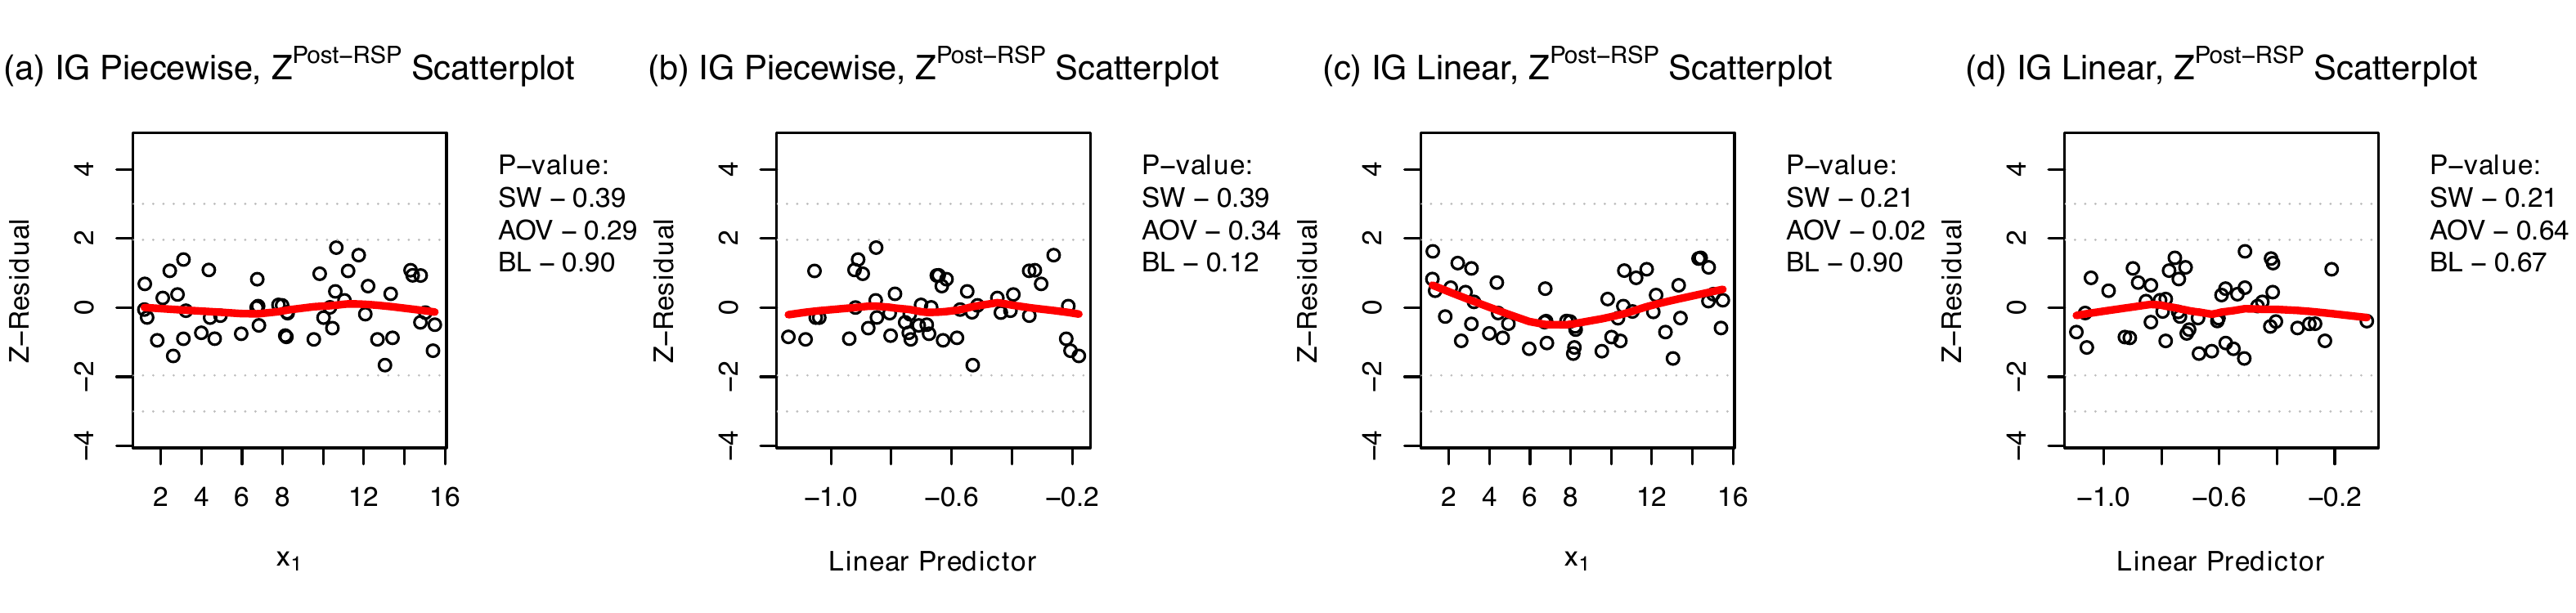
\includegraphics[keepaspectratio]{plot/piecewise_ig_fig_n50.png}}
\end{center}

\begin{itemize}
\tightlist
\item
  \textbf{Correct Model (a)(b)}: No trend against \(X_1\) or fitted
  values.
\item
  \textbf{Misspecified Model (c)(d):} Clear nonlinear pattern against
  \(X_1\) (c), but masked when plotted against the overall linear
  predictor (d). \emph{Covariate-specific plots are essential.}
\end{itemize}
\end{frame}

\begin{frame}{Empirical \(p\)-value Distributions (IG)}
\protect\phantomsection\label{empirical-p-value-distributions-ig}
\begin{center}
\pandocbounded{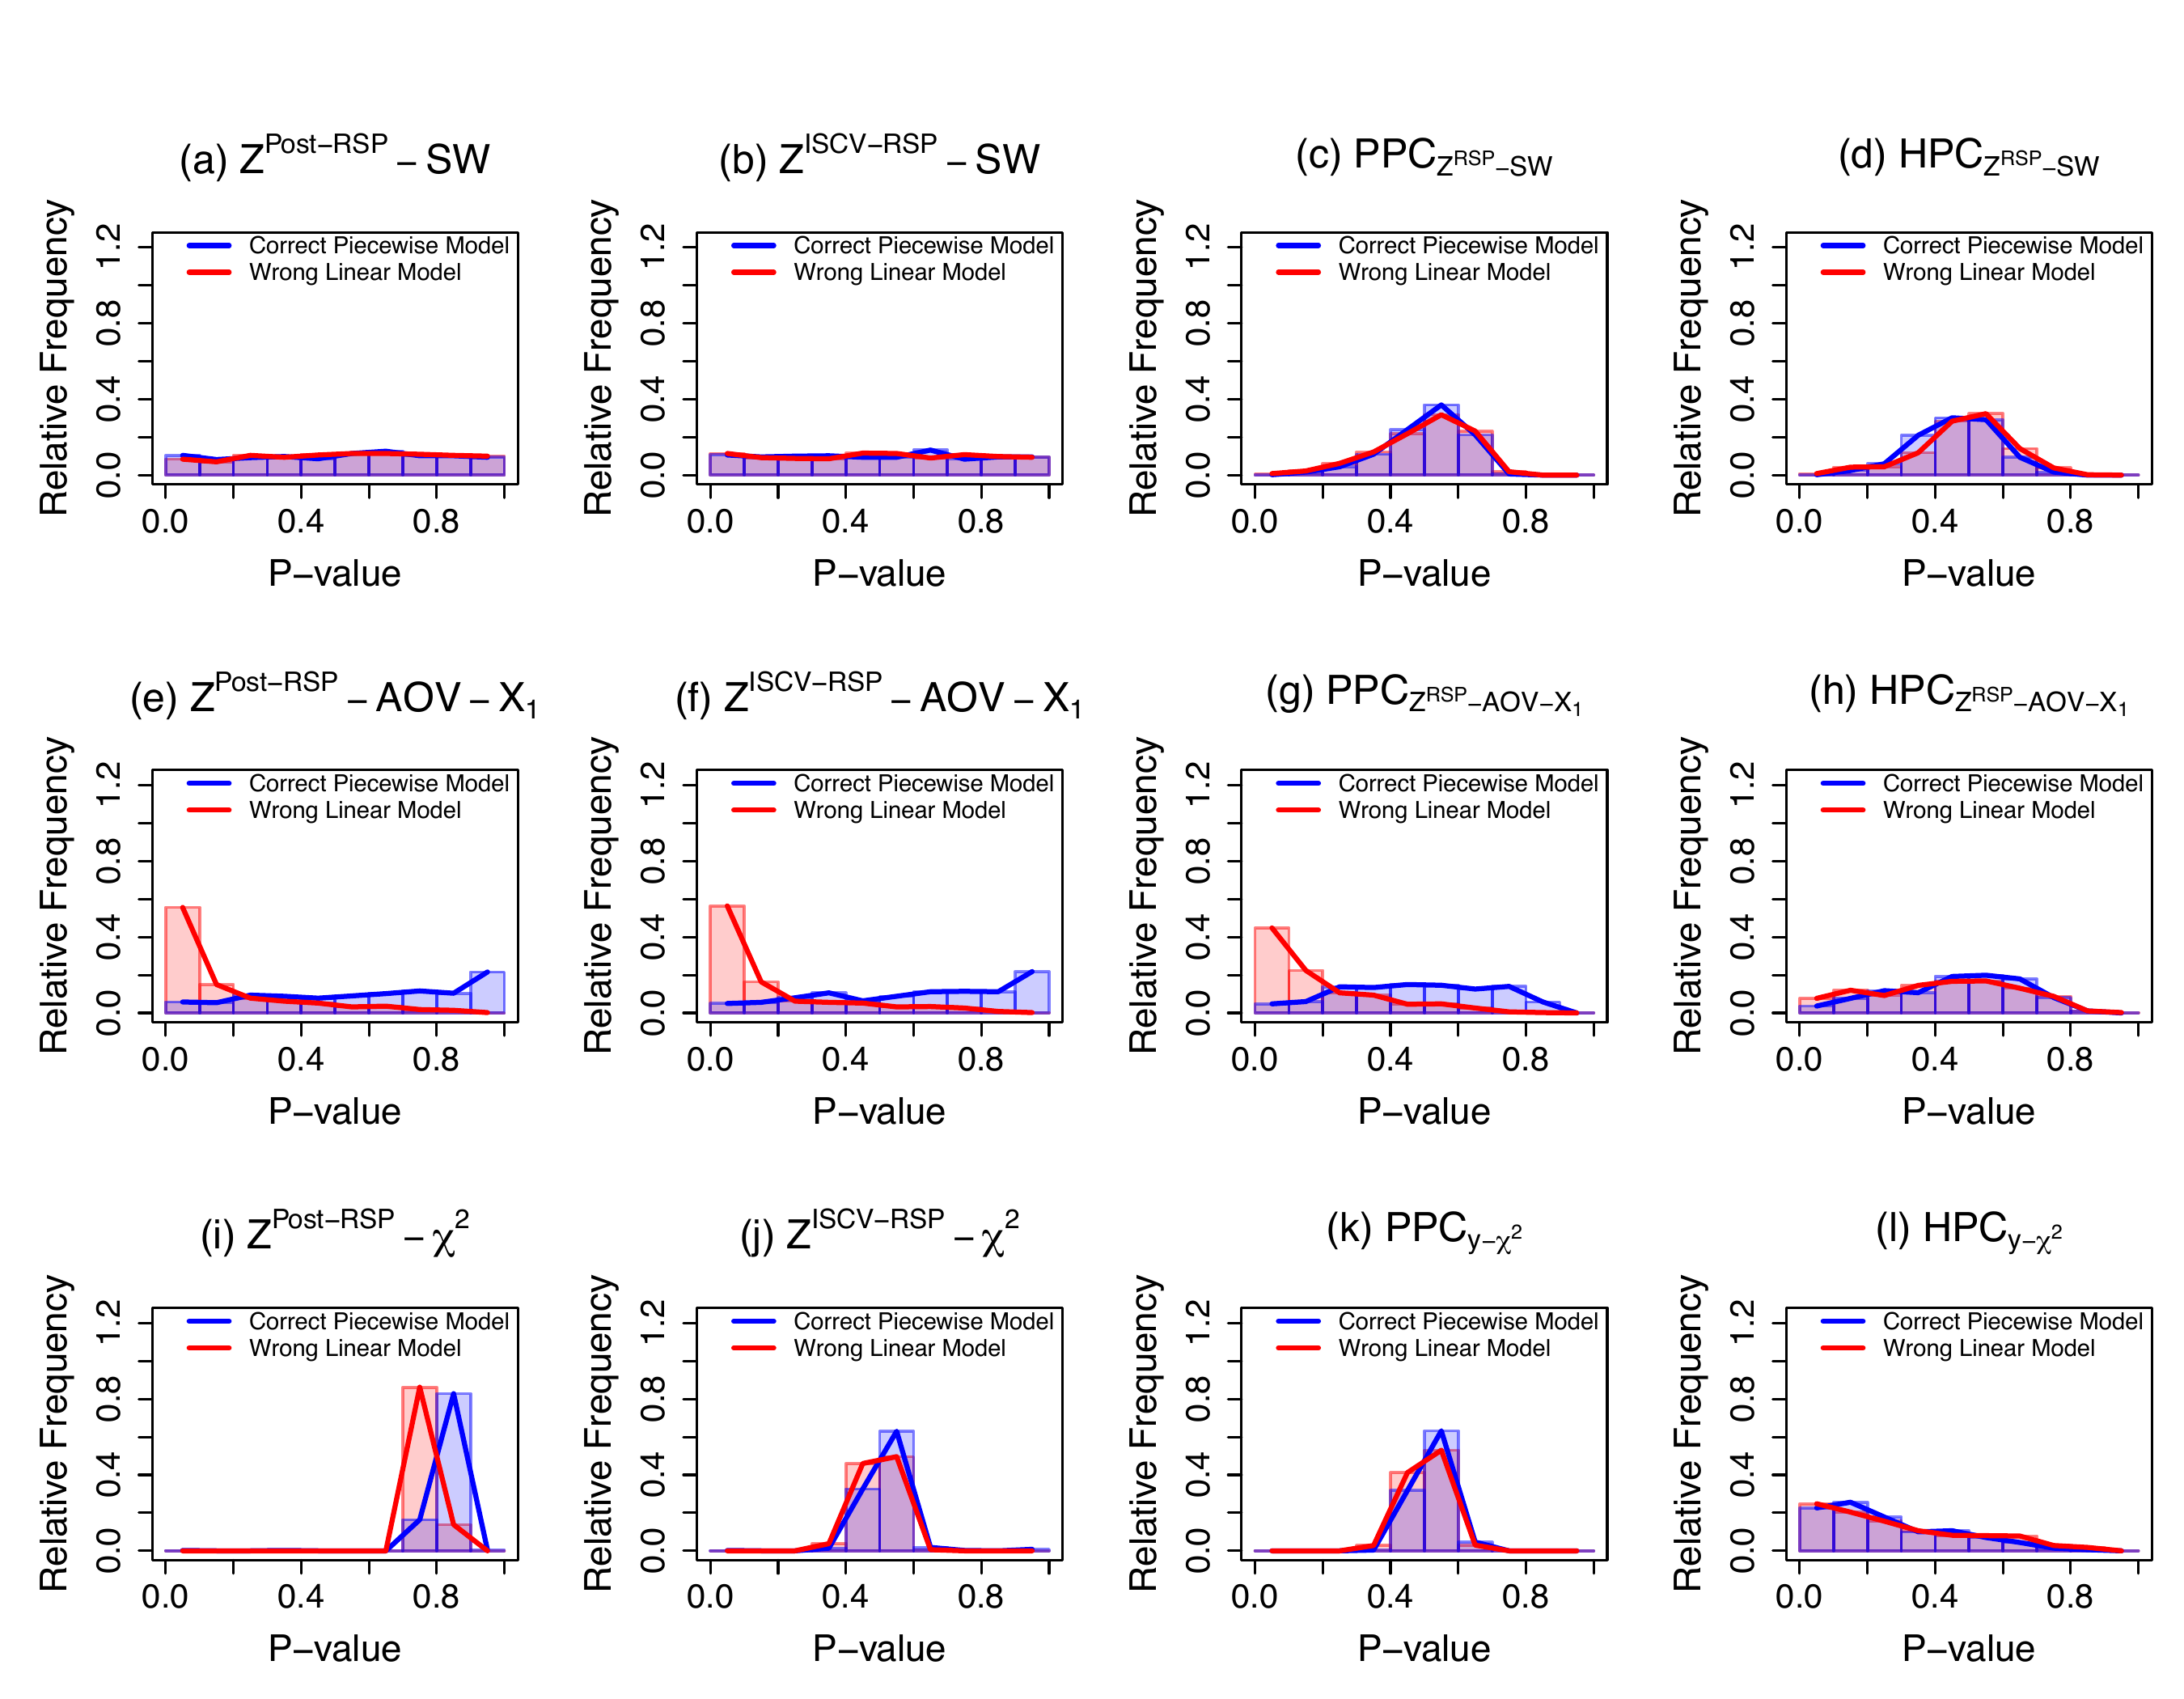
\includegraphics[keepaspectratio]{plot/piecewise_combined_histograms_n50.png}}
\end{center}

\begin{itemize}
\tightlist
\item
  \textbf{Blue = Correct Model, Red = Misspecified Model.}
\item
  Z-residual AOV tests (e, f) are uniform under correct model, strongly
  concentrated near zero under wrong model. SW/\(\chi^2\) lack power.
\end{itemize}
\end{frame}

\begin{frame}{Rejection Rates \& Power (IG)}
\protect\phantomsection\label{rejection-rates-power-ig}
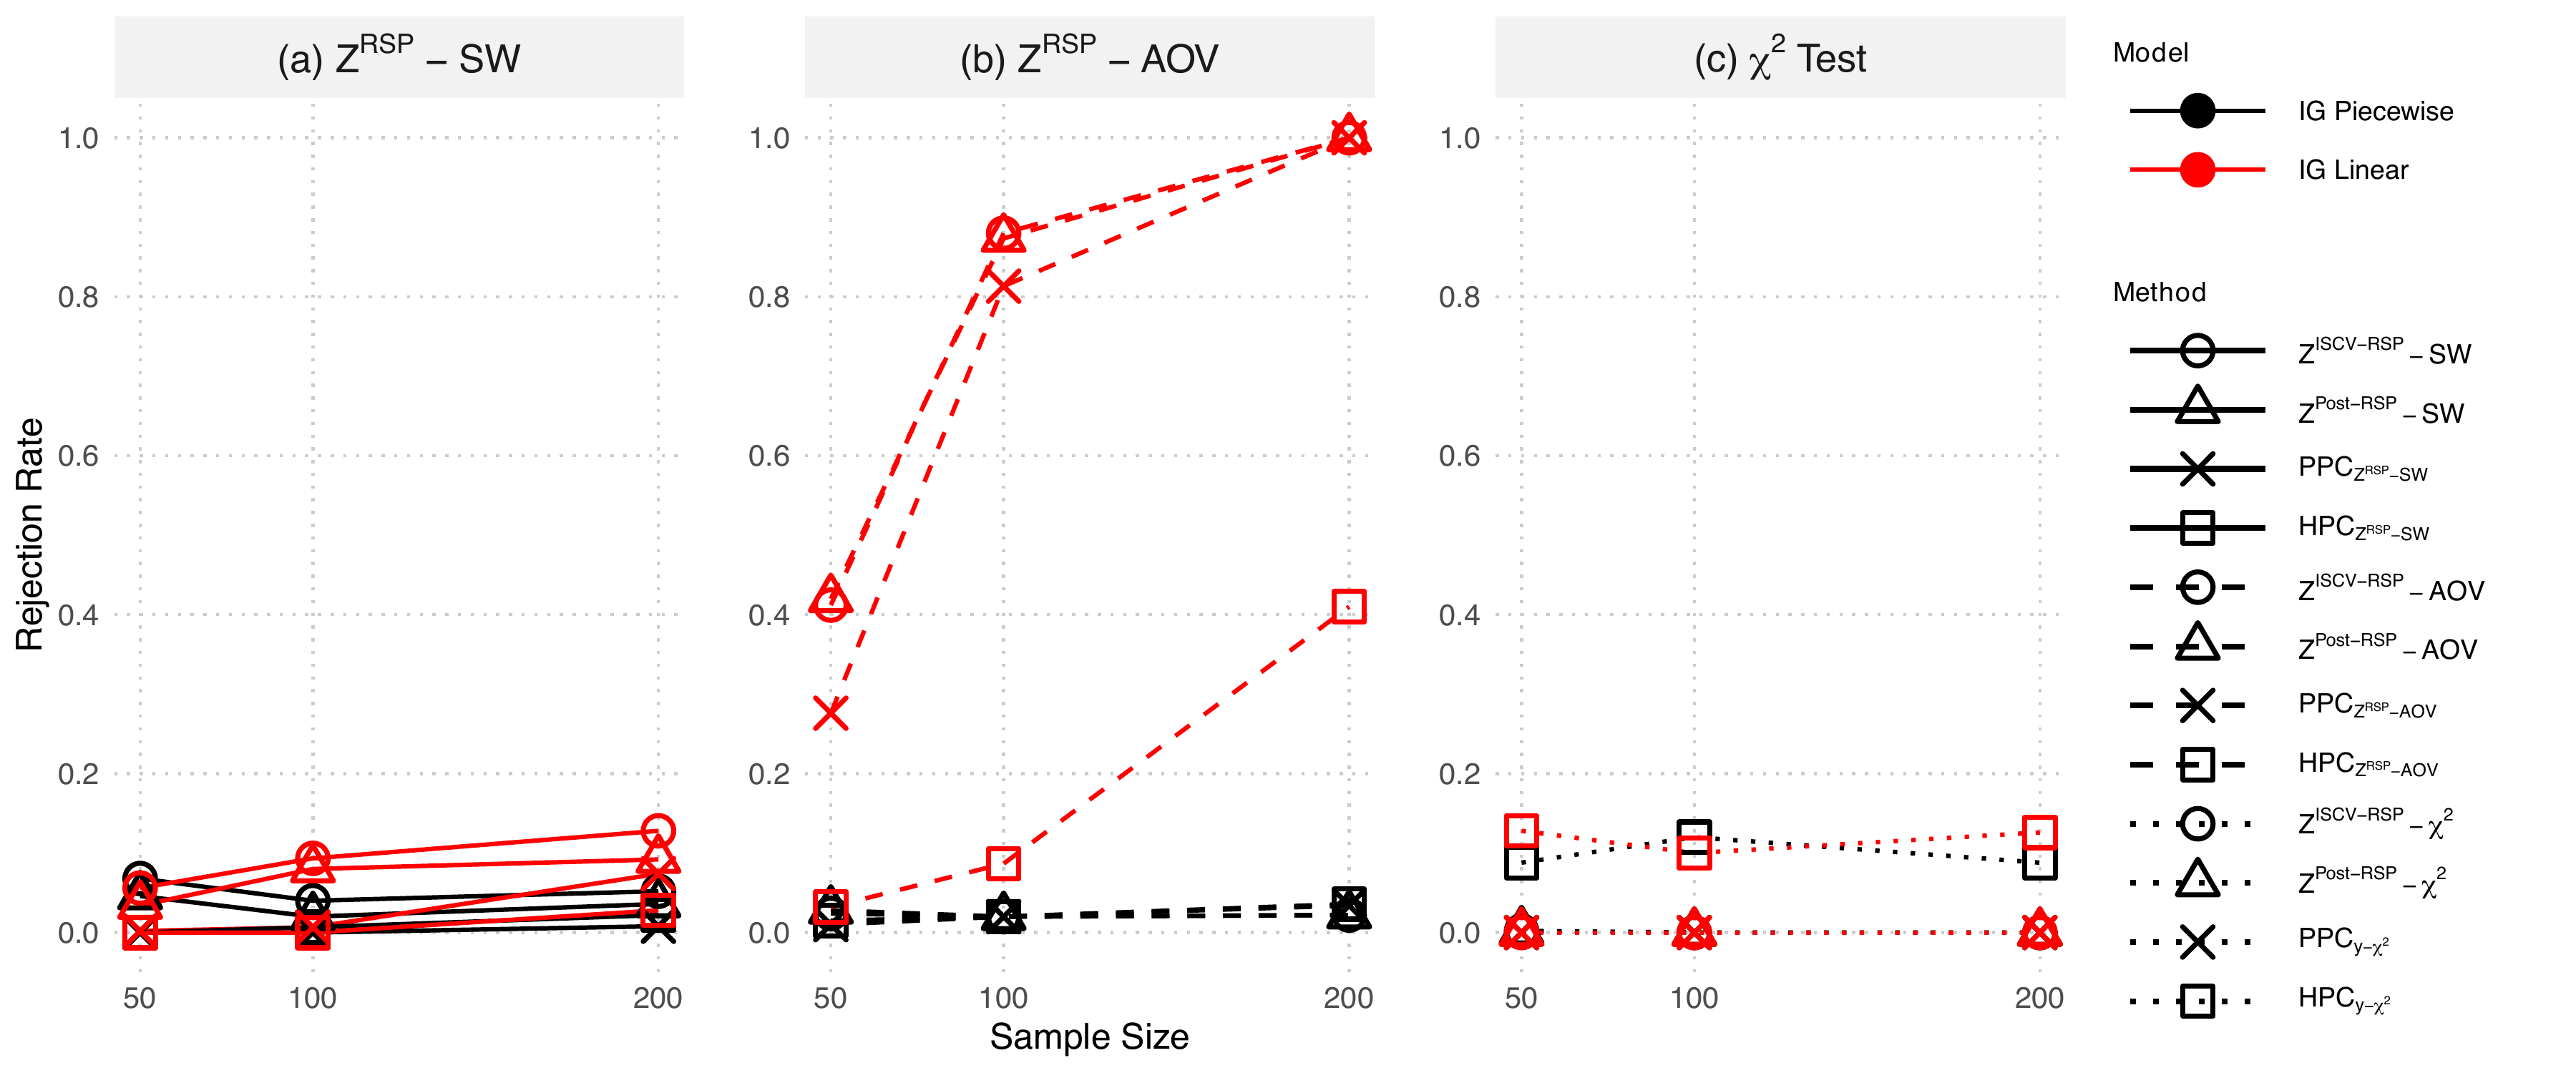
\includegraphics[width=1\linewidth,height=\textheight,keepaspectratio]{plot/piecewise_rejection_rate_plot.png}

\begin{itemize}
\tightlist
\item
  Z-AOV (b) maintains nominal \(\alpha=0.05\) (black) and achieves
  rapidly increasing power (red) as \(n\) grows.
\item
  Traditional SW (a) and \(\chi^2\) (c) fail to detect localized mean
  misspecification.
\end{itemize}
\end{frame}

\begin{frame}{Simulation 2: Hurdle Negative Binomial (HNB)}
\protect\phantomsection\label{simulation-2-hurdle-negative-binomial-hnb}
\begin{itemize}
\tightlist
\item
  \textbf{Setup:} Discrete count data with excess zeros
  (\(\approx 30\%\)). \(n \in \{50, 100, 200\}\). Requires auxiliary
  randomization \(U\).
\item
  \textbf{DGP:} True model has a logarithmic effect \(\log(X_1)\) in the
  count component.
\item
  \textbf{Fitted Models:}

  \begin{enumerate}
  \tightlist
  \item
    \textbf{Correct:} Logarithmic HNB.
  \item
    \textbf{Misspecified:} Linear HNB.
  \end{enumerate}
\item
  \textbf{Goal:} Detect nonlinear mean misspecification in zero-inflated
  count data.
\end{itemize}
\end{frame}

\begin{frame}{Visual Diagnostics (HNB, \(n=50\))}
\protect\phantomsection\label{visual-diagnostics-hnb-n50}
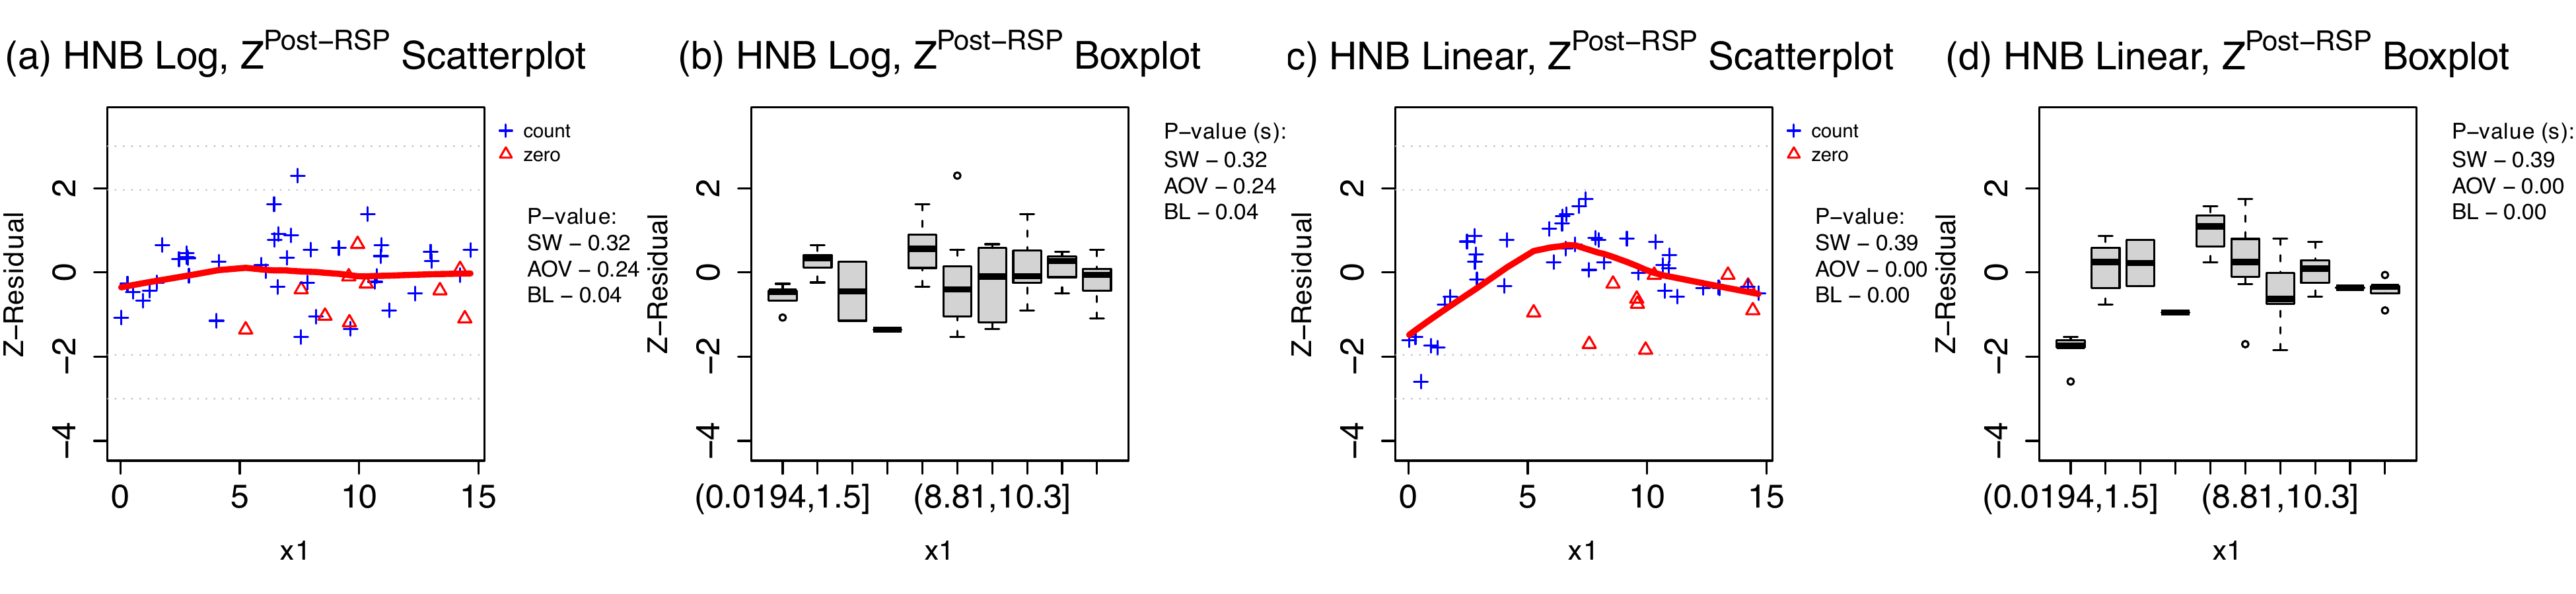
\includegraphics[width=0.8\linewidth,height=\textheight,keepaspectratio]{plot/sim2_HNB_scatter_box_plot.png}

\begin{itemize}
\tightlist
\item
  \textbf{Top (Correct):} Residuals scattered, boxplots homogeneous
  across \(X_1\) bins.
\item
  \textbf{Bottom (Misspecified):} Pronounced grouped mean differences
  across \(X_1\). Detected by AOV grouped test.
\end{itemize}
\end{frame}

\begin{frame}{Empirical \(p\)-value Distributions (HNB)}
\protect\phantomsection\label{empirical-p-value-distributions-hnb}
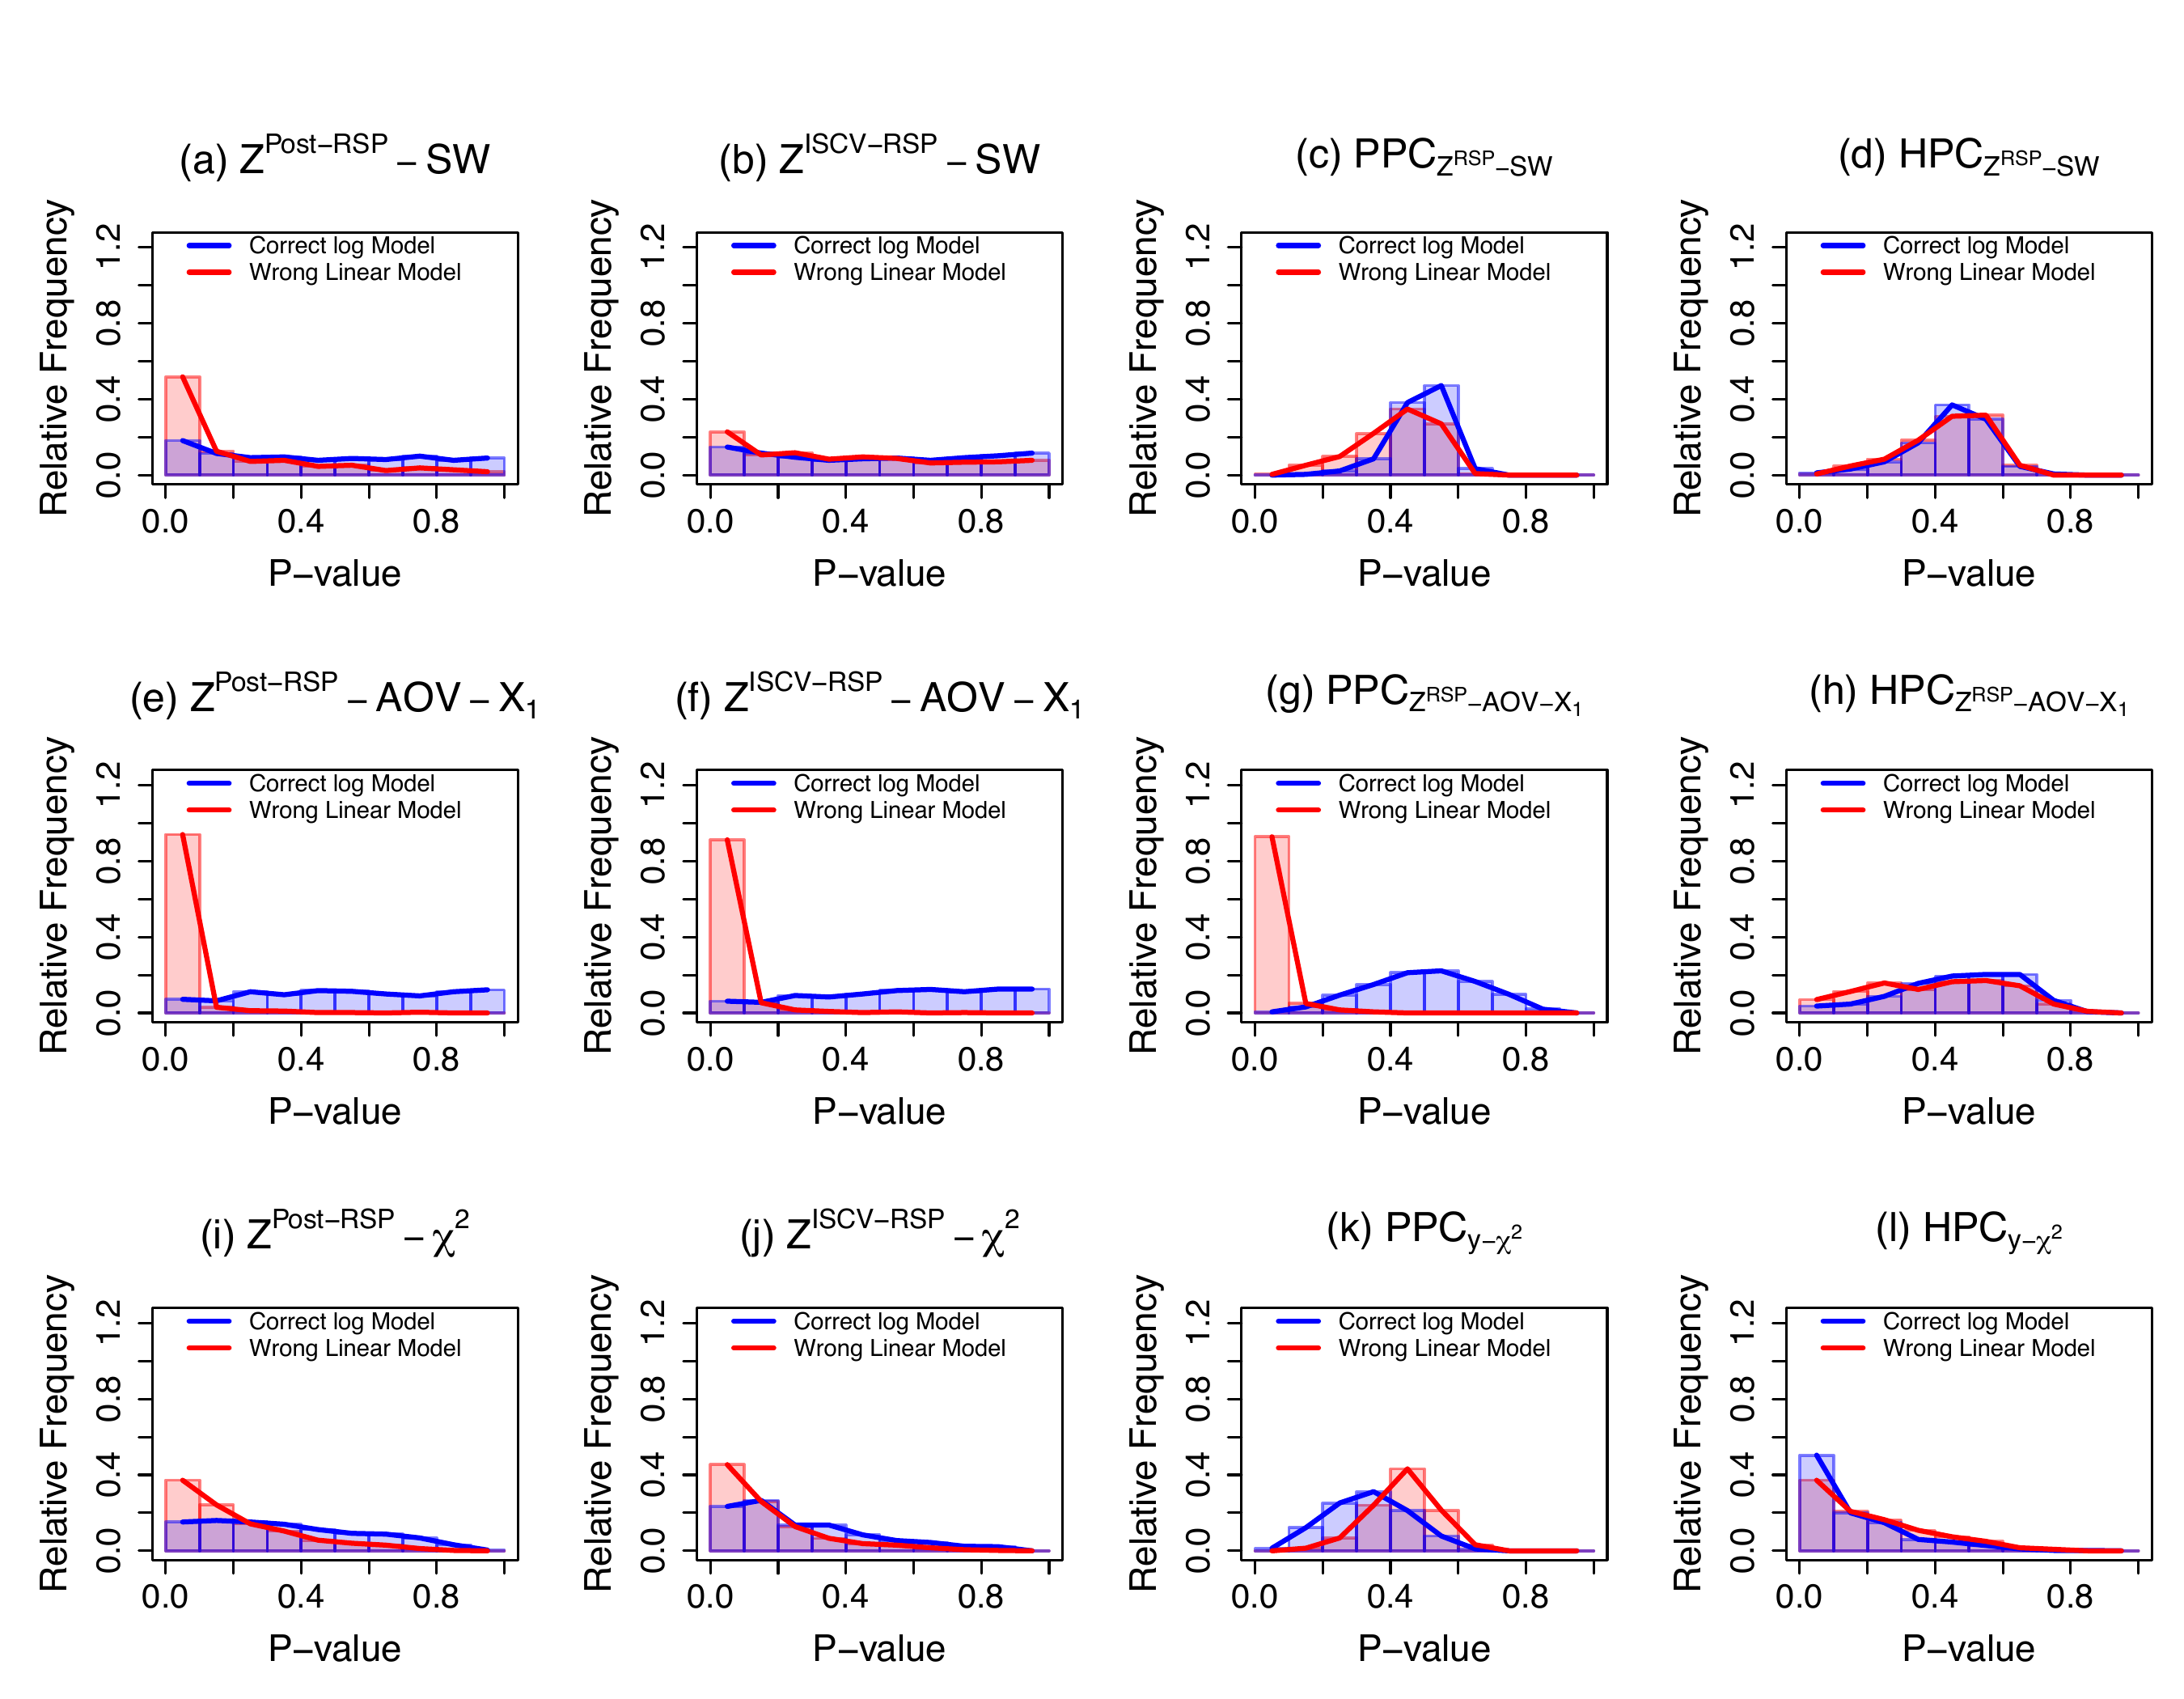
\includegraphics[width=0.7\linewidth,height=\textheight,keepaspectratio]{plot/sim2_hnb_combined_histograms_n50.png}

\begin{itemize}
\tightlist
\item
  AOV tests (e, f) based on posterior/ISCV Z-residuals remain well
  calibrated (blue) and highly powerful (red). PPC and HPC methods
  cluster near \(0.5\) under the null.
\end{itemize}
\end{frame}

\begin{frame}{Rejection Rates \& Power (HNB)}
\protect\phantomsection\label{rejection-rates-power-hnb}
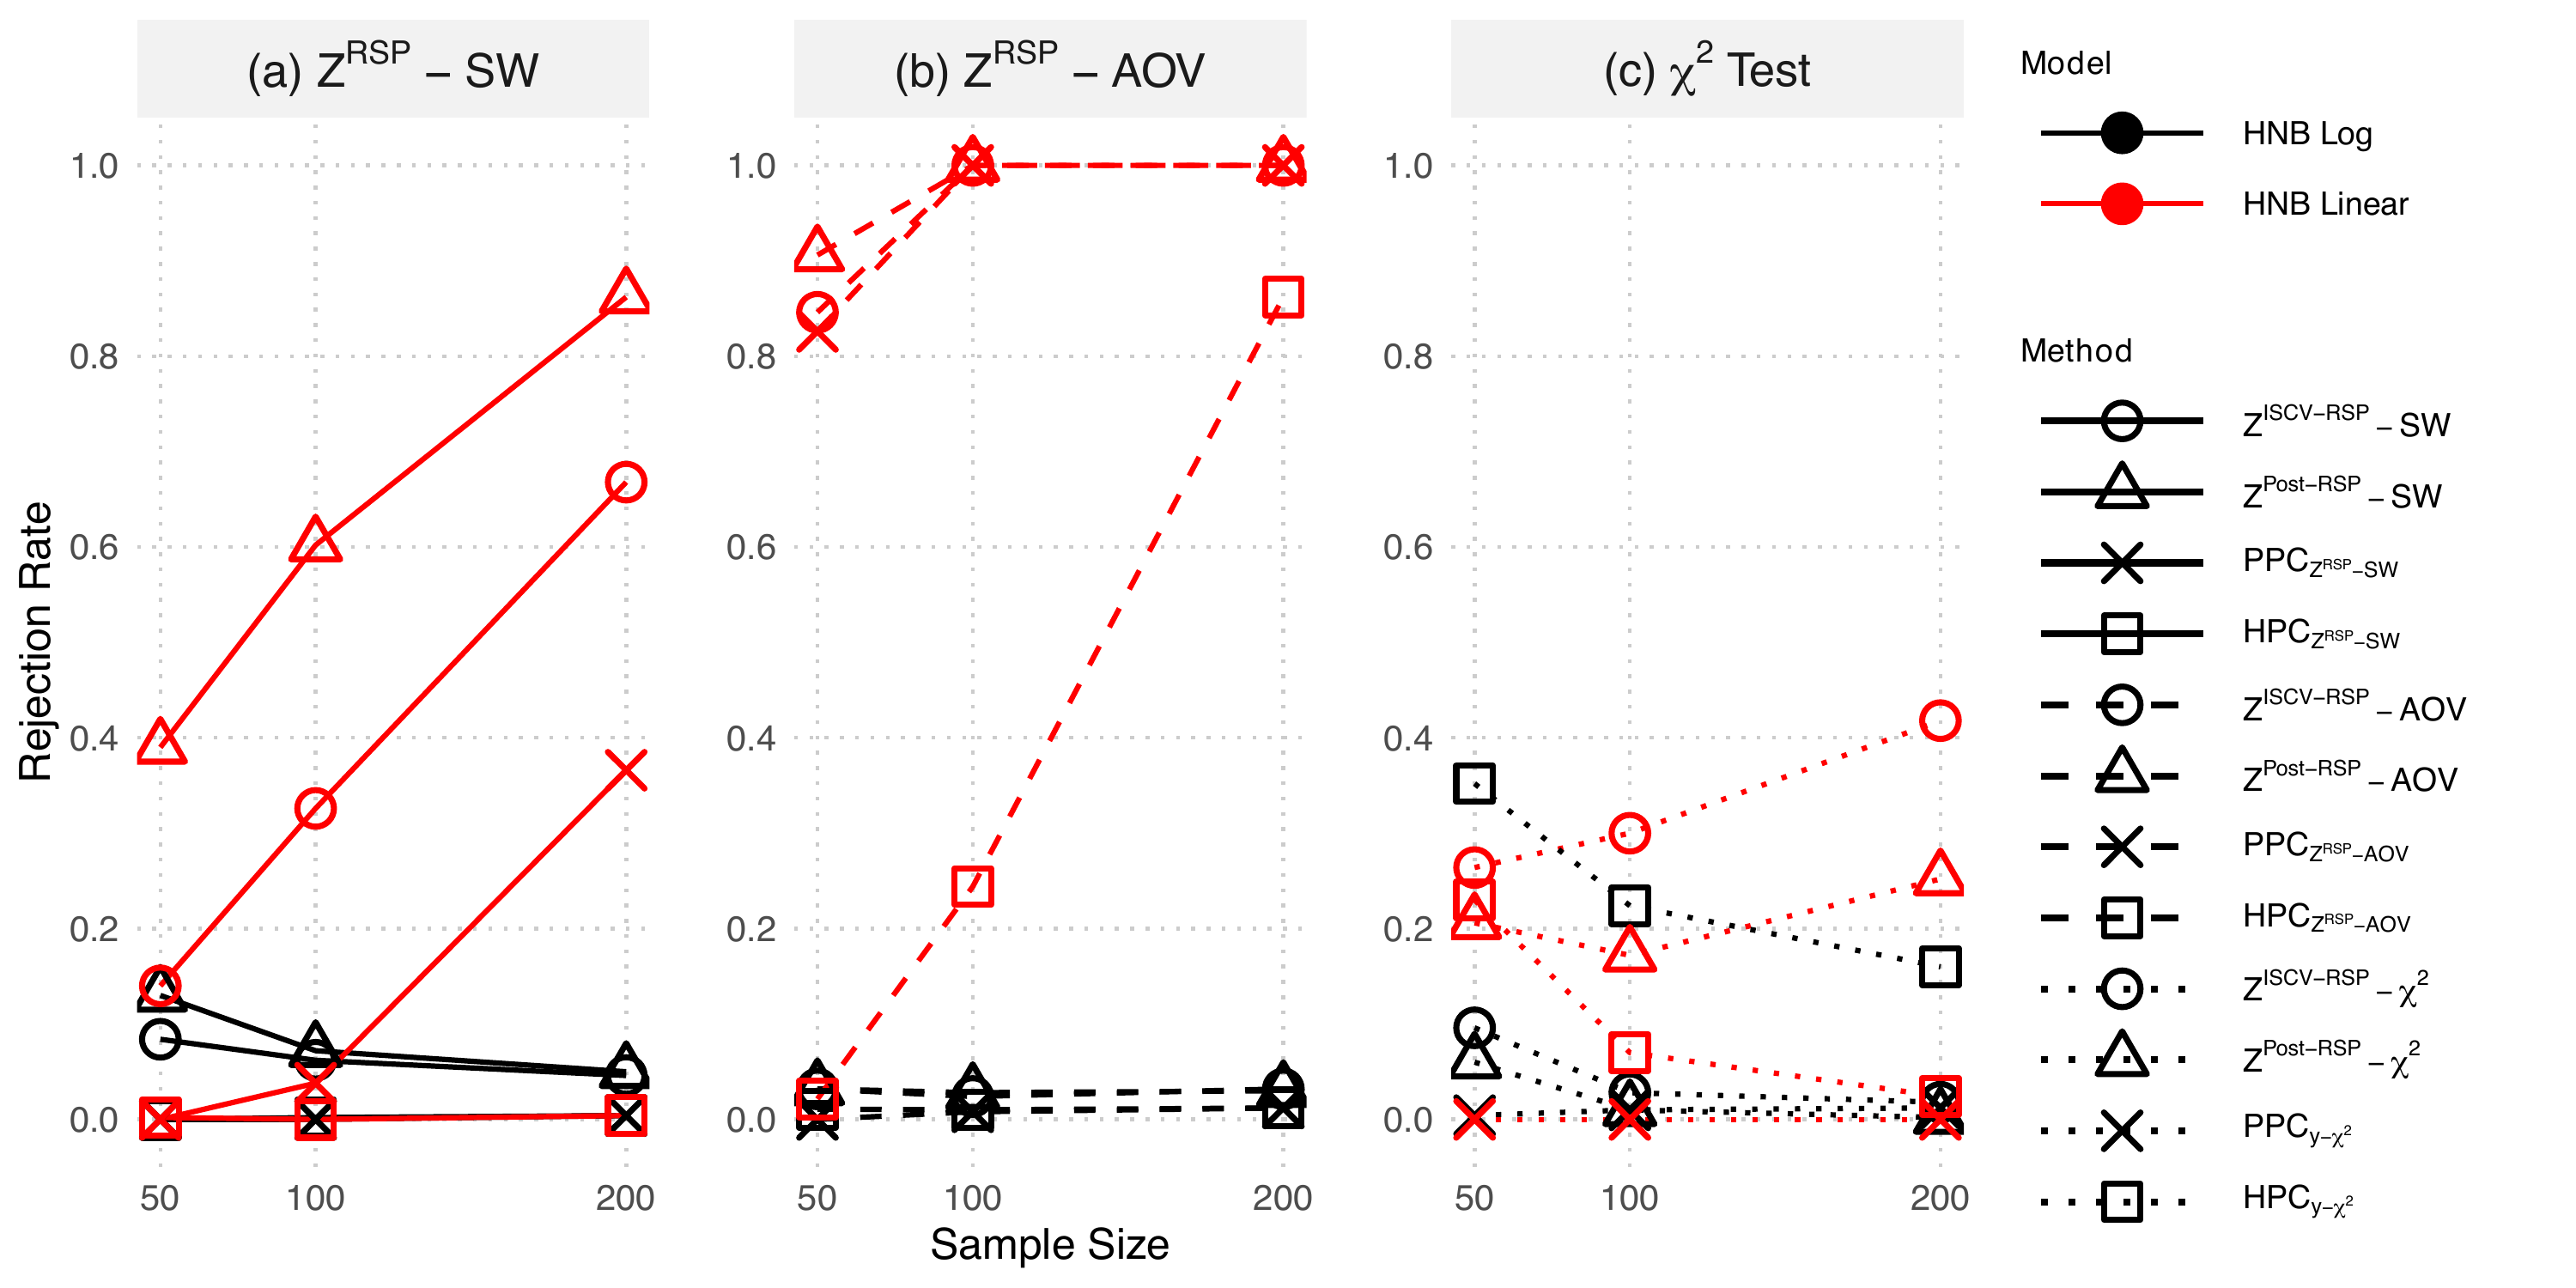
\includegraphics[width=1\linewidth,height=\textheight,keepaspectratio]{plot/sim2_hurdle_nl_rejection_rate_plot.png}

\begin{itemize}
\tightlist
\item
  Z-AOV maintains low Type-I error rates (black) and achieves nearly
  \(100\%\) power for \(n \ge 100\) (red). PPC AOV performs well but
  lags at smaller sample sizes.
\end{itemize}
\end{frame}

\section{4. Real-World Application}\label{real-world-application}

\begin{frame}{Dolphin-Sighting Dataset}
\protect\phantomsection\label{dolphin-sighting-dataset}
\begin{itemize}
\tightlist
\item
  \textbf{Data:} \(n=936\) observations, estuarine--coastal gradient.
\item
  \textbf{Response:} Count of dolphin sightings (extremely sparse,
  \(\sim 75\%\) zeros).
\item
  \textbf{Covariates:} Water depth, temperature, distance to river
  mouth, salinity, turbidity, year, location.
\item
  \textbf{Initial Strategy:} Fit linear models across 4 families:

  \begin{itemize}
  \tightlist
  \item
    Hurdle Poisson, Hurdle Negative Binomial (HNB)
  \item
    Poisson, Negative Binomial (NB)
  \end{itemize}
\end{itemize}
\end{frame}

\begin{frame}{Overall Goodness-of-Fit (Linear Models)}
\protect\phantomsection\label{overall-goodness-of-fit-linear-models}
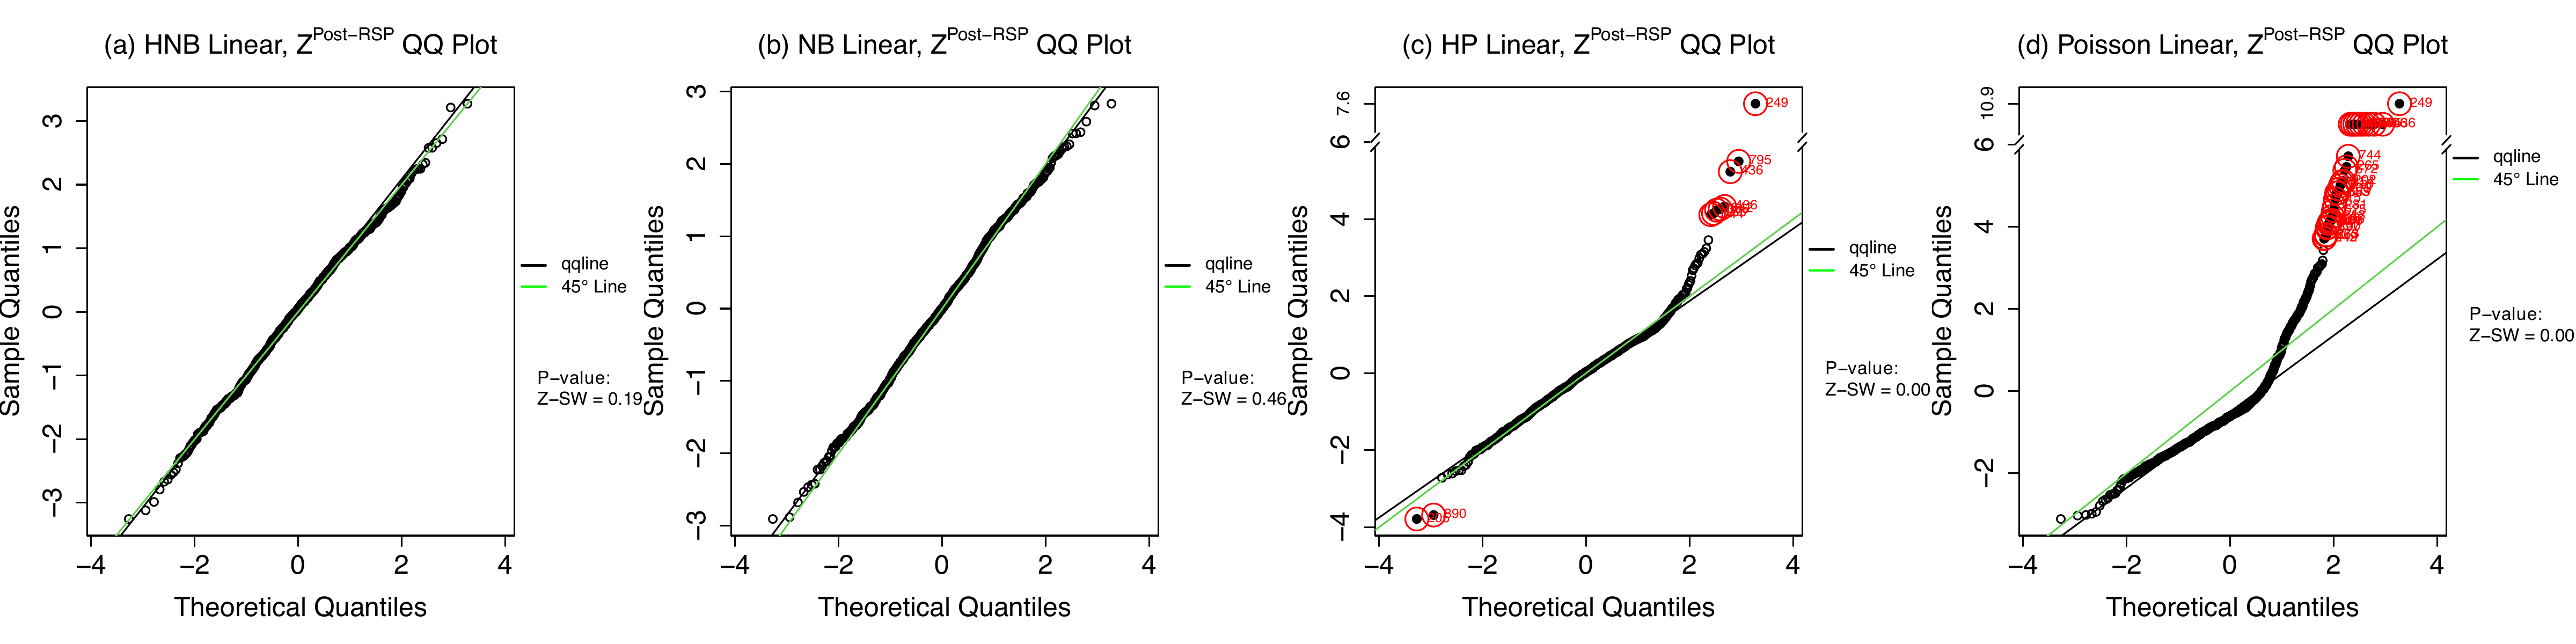
\includegraphics[width=1\linewidth,height=\textheight,keepaspectratio]{plot/realdata_qqplot.png}

\begin{itemize}
\tightlist
\item
  \textbf{Result:} HNB (a) and NB (b) show adequate overall fit
  (adhering to diagonal, SW \(p \ge 0.05\)). Poisson models (c, d) fail
  dramatically due to unmodeled overdispersion.
\end{itemize}
\end{frame}

\begin{frame}[fragile]{Detecting Nonlinearity in Depth}
\protect\phantomsection\label{detecting-nonlinearity-in-depth}
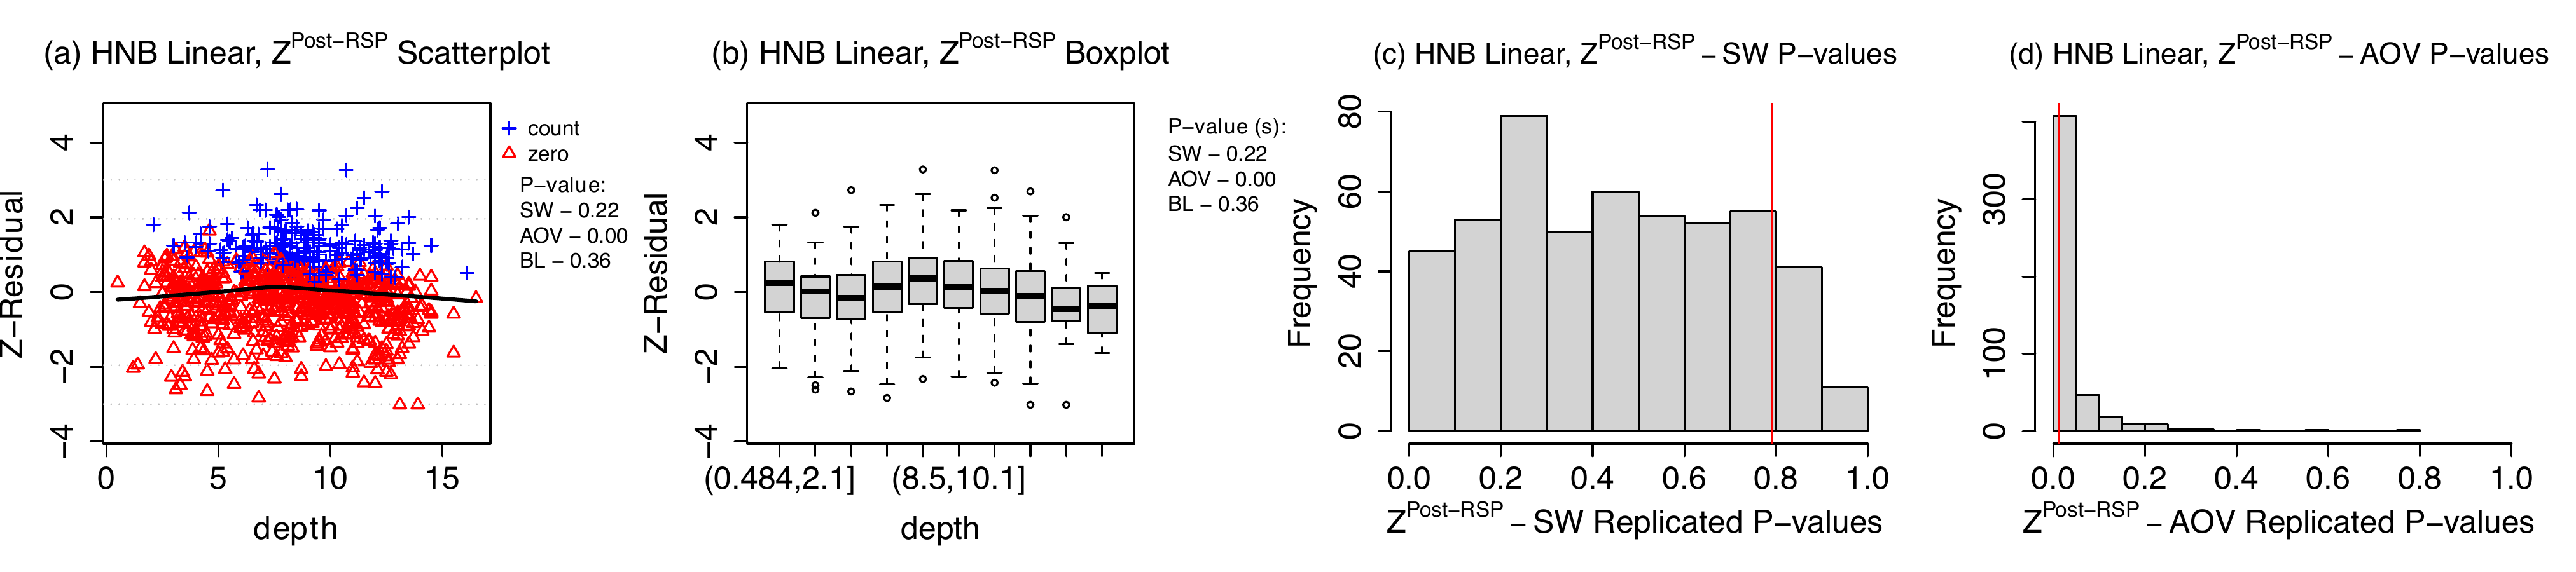
\includegraphics[width=0.7\linewidth,height=\textheight,keepaspectratio]{plot/realdata_plot_linear.png}

\begin{itemize}
\tightlist
\item
  Plotting linear HNB Z-residuals against \texttt{depth} reveals a clear
  \textbf{U-shape} (a) and heterogeneous grouped boxplots (b).
\item
  AOV test confirms severe non-linearity (median upper-bound \(p\)-value
  = \(0.012\)).
\end{itemize}
\end{frame}

\begin{frame}[fragile]{The Refined Nonlinear Model}
\protect\phantomsection\label{the-refined-nonlinear-model}
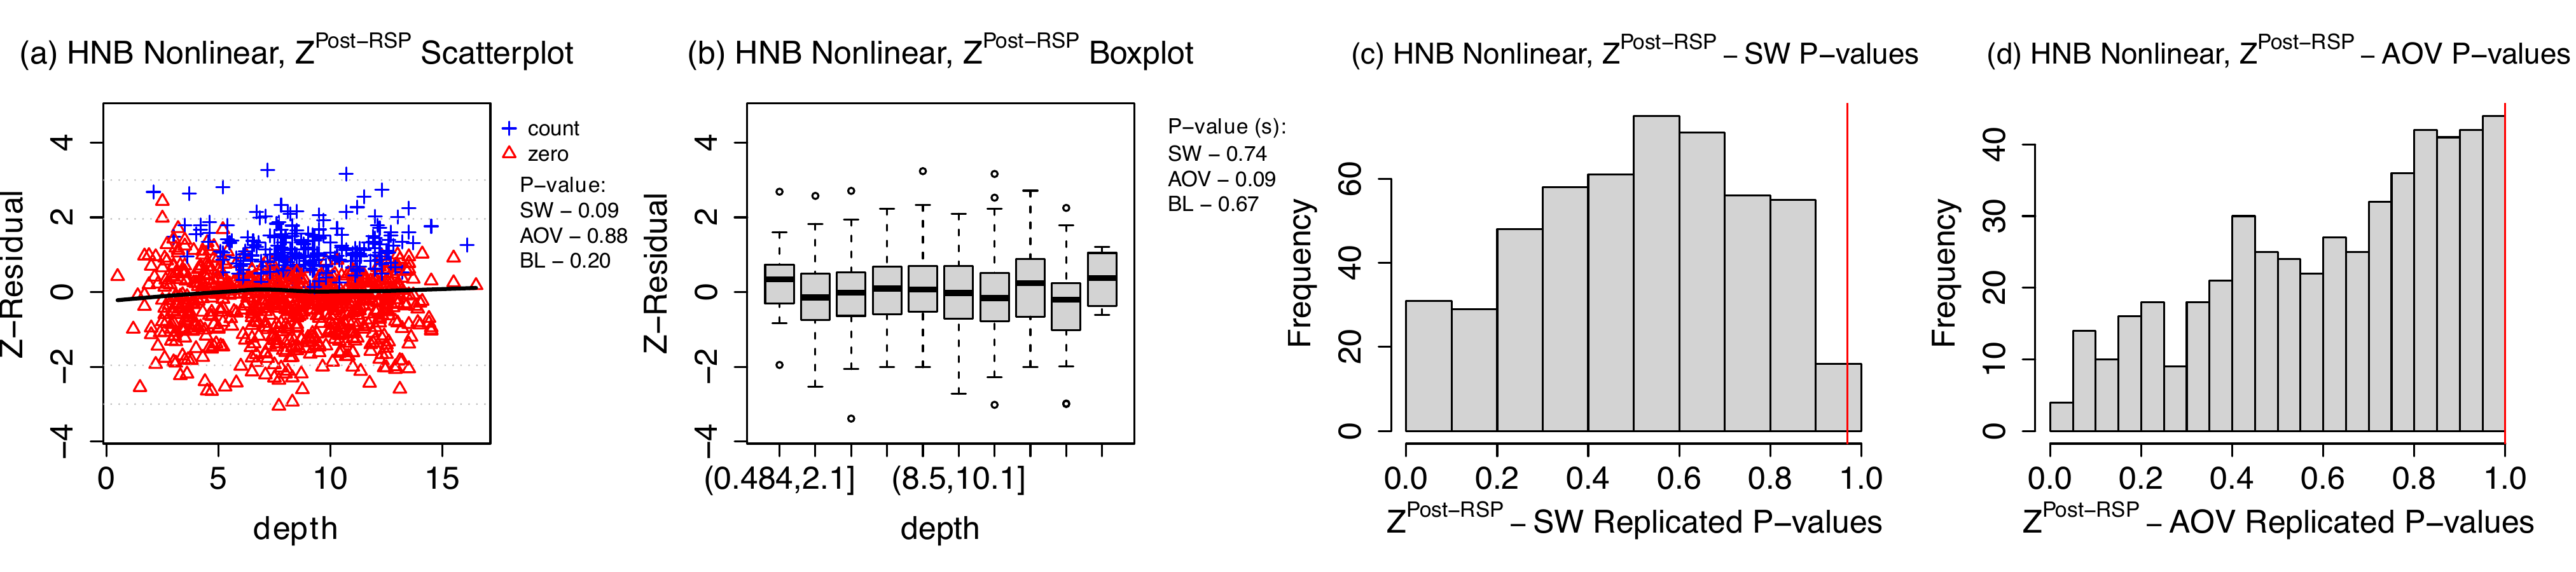
\includegraphics[width=0.7\linewidth,height=\textheight,keepaspectratio]{plot/realdata_plot_nonlinear.png}

\begin{itemize}
\tightlist
\item
  \textbf{Refinement:} Added piecewise quadratic effect for
  \texttt{depth} based on visual turning point at 7.95m.
\item
  \textbf{Result:} Patterns eliminated. Scatterplot and boxplots are
  homogeneous. AOV test \(p\)-value climbs to \(1.00\).
\end{itemize}
\end{frame}

\begin{frame}{Model Comparison}
\protect\phantomsection\label{model-comparison}
{\def\LTcaptype{none} % do not increment counter
\begin{longtable}[]{@{}
  >{\raggedright\arraybackslash}p{(\linewidth - 8\tabcolsep) * \real{0.2000}}
  >{\raggedright\arraybackslash}p{(\linewidth - 8\tabcolsep) * \real{0.2000}}
  >{\raggedright\arraybackslash}p{(\linewidth - 8\tabcolsep) * \real{0.2000}}
  >{\raggedright\arraybackslash}p{(\linewidth - 8\tabcolsep) * \real{0.2000}}
  >{\raggedright\arraybackslash}p{(\linewidth - 8\tabcolsep) * \real{0.2000}}@{}}
\toprule\noalign{}
\begin{minipage}[b]{\linewidth}\raggedright
Family
\end{minipage} & \begin{minipage}[b]{\linewidth}\raggedright
Model Type
\end{minipage} & \begin{minipage}[b]{\linewidth}\raggedright
Z-SW \(p\)
\end{minipage} & \begin{minipage}[b]{\linewidth}\raggedright
Z-AOV \(p\)
\end{minipage} & \begin{minipage}[b]{\linewidth}\raggedright
\(\Delta_{\text{elpd}}\) (LOO)
\end{minipage} \\
\midrule\noalign{}
\endhead
\textbf{HNB} & \textbf{Nonlinear} & \(1.000\) & \(1.000\) &
\textbf{\(0.0\)} \\
HNB & Linear & \(0.790\) & \(0.012\) & \(-19.9\) \\
NB & Nonlinear & \(0.337\) & \(0.760\) & \(-34.0\) \\
NB & Linear & \(0.299\) & \(0.010\) & \(-42.5\) \\
HP & Linear & \(<0.01\) & \(0.020\) & \(-118.6\) \\
\bottomrule\noalign{}
\end{longtable}
}

\begin{itemize}
\tightlist
\item
  The \textbf{Nonlinear HNB} model satisfies all diagnostic checks and
  significantly outperforms all other models out-of-sample.
\item
  The nonlinear effect primarily acts on the \emph{hurdle} component
  (zero-inflation probability increases away from 7.95m depth).
\end{itemize}
\end{frame}

\section{5. Conclusion \& Future
Directions}\label{conclusion-future-directions}

\begin{frame}{Summary of Contributions}
\protect\phantomsection\label{summary-of-contributions}
\begin{itemize}
\tightlist
\item
  \textbf{Methodological Shift:} Transitioned from ``test-first, then
  summarize'' (PPC) to ``summarize-first, then test'' (Z-residuals).
\item
  \textbf{Asymptotic Calibration:} Posterior and ISCV Z-residuals
  converge to standard normal, ensuring well-calibrated \(p\)-values.
\item
  \textbf{Diagnostic Versatility:} Enables targeted tests (AOV, SW) that
  uncover structural flaws (like functional form misspecification) which
  omnibus checks miss.
\item
  \textbf{Preserved Power:} Uses full sample size without holdout
  reductions.
\end{itemize}
\end{frame}

\begin{frame}{Limitations \& Future Directions}
\protect\phantomsection\label{limitations-future-directions}
\begin{itemize}
\tightlist
\item
  \textbf{Limitations:}

  \begin{itemize}
  \tightlist
  \item
    Strict observation-level focus: Insensitive to internal/latent
    structure misspecifications (hierarchical effects, priors).
  \end{itemize}
\item
  \textbf{Future Work:}

  \begin{itemize}
  \tightlist
  \item
    Extend framework to internal model components (synergizing with
    Uniform Parametrization Checks).
  \item
    Expand the suite of targeted Z-residual tests (e.g., spatial
    dependence, formal e-values for multiple testing correction).
  \item
    Improve computational efficiency for summarizing simulated
    \(p\)-values over auxiliary \(\mathbf{U}\).
  \end{itemize}
\end{itemize}
\end{frame}

\begin{frame}{Questions?}
\protect\phantomsection\label{questions}
\textbf{Thank you.}

\emph{Paper: ``Z-residuals: A Versatile Diagnostic Framework for
Bayesian Models''}
\end{frame}




\end{document}
